%%%%%%%%%%%%%%%%%%%%%%%%%%%%%%%%%%%%%%%%%%%%%%%%%%%
%% LaTeX book template                           %%
%% Author:  Amber Jain (http://amberj.devio.us/) %%
%% License: ISC license                          %%
%%%%%%%%%%%%%%%%%%%%%%%%%%%%%%%%%%%%%%%%%%%%%%%%%%%
% Source: http://tex.stackexchange.com/a/8584/5645

\documentclass[a4paper,11pt]{book}
\usepackage{pgfplots}

\usepackage[T1]{fontenc}
\usepackage[utf8]{inputenc}
\usepackage{lmodern}
%%%%%%%%%%%%%%%%%%%%%%%%%%%%%%%%%%%%%%%%%%%%%%%%%%%%%%%%%
% Source: http://en.wikibooks.org/wiki/LaTeX/Hyperlinks %
%%%%%%%%%%%%%%%%%%%%%%%%%%%%%%%%%%%%%%%%%%%%%%%%%%%%%%%%%
\usepackage{hyperref}
\usepackage{graphicx}
\usepackage[english]{babel}


%%%%%%%%%%%%%%%%%%%%%%%%%%%%%%%%%%%%%%%%%%%%%%%%%%%%%%%%%%%%%%%%%%%%%%%%%%%%%%%%
% 'dedication' environment: To add a dedication subsubsection at the start of book %
% Source: http://www.tug.org/pipermail/texhax/2010-June/015184.html            %
%%%%%%%%%%%%%%%%%%%%%%%%%%%%%%%%%%%%%%%%%%%%%%%%%%%%%%%%%%%%%%%%%%%%%%%%%%%%%%%%
\newenvironment{dedication}
{
   \cleardoublepage
   \thispagestyle{empty}
   \vspace*{\stretch{1}}
   \hfill\begin{minipage}[t]{0.66\textwidth}
   \raggedright
}
{
   \end{minipage}
   \vspace*{\stretch{3}}
   \clearpage
}

%%%%%%%%%%%%%%%%%%%%%%%%%%%%%%%%%%%%%%%%%%%%%%%%
% Chapter quote at the start of chapter        %
% Source: http://tex.stackexchange.com/a/53380 %
%%%%%%%%%%%%%%%%%%%%%%%%%%%%%%%%%%%%%%%%%%%%%%%%
\makeatletter
\renewcommand{\@chapapp}{}% Not necessary...
\newenvironment{chapquote}[2][2em]
  {\setlength{\@tempdima}{#1}%
   \def\chapquote@author{#2}%
   \parshape 1 \@tempdima \dimexpr\textwidth-2\@tempdima\relax%
   \itshape}
  {\par\normalfont\hfill--\ \chapquote@author\hspace*{\@tempdima}\par\bigskip}
\makeatother

%%%%%%%%%%%%%%%%%%%%%%%%%%%%%%%%%%%%%%%%%%%%%%%%%%%
% First page of book which contains 'stuff' like: %
%  - Book title, subtitle                         %
%  - Book author name                             %
%%%%%%%%%%%%%%%%%%%%%%%%%%%%%%%%%%%%%%%%%%%%%%%%%%%

% Book's title and subtitle
\title{\Huge \textbf{Proyecto Final}
 \footnote{This is a footnote.} \\ \huge Minería de Datos \footnote{This is yet another footnote.}}
% Author
\author{\textsc{David Jiménez}}


  

\begin{document}

\frontmatter
\maketitle

%%%%%%%%%%%%%%%%%%%%%%%%%%%%%%%%%%%%%%%%%%%%%%%%%%%%%%%%%%%%%%%
% Add a dedication subsubsection to dedicate your book to someone %
%%%%%%%%%%%%%%%%%%%%%%%%%%%%%%%%%%%%%%%%%%%%%%%%%%%%%%%%%%%%%%%
%\begin{dedication}
%Dedicado a mi.
%\end{dedication}

%%%%%%%%%%%%%%%%%%%%%%%%%%%%%%%%%%%%%%%%%%%%%%%%%%%%%%%%%%%%%%%%%%%%%%%%
% Auto-generated table of contents, list of figures and list of tables %
%%%%%%%%%%%%%%%%%%%%%%%%%%%%%%%%%%%%%%%%%%%%%%%%%%%%%%%%%%%%%%%%%%%%%%%%




\tableofcontents

\listoffigures
\listoftables

\mainmatter

%%%%%%%%%%%
% Resumen %
%%%%%%%%%%%
\section*{{\Huge Resumen}}
\addcontentsline{toc}{section}{\protect\numberline{}Resumen}%

%%%%%%%%%%%%%%%%%%%%%
%Sección del Resumen%
%%%%%%%%%%%%%%%%%%%%%
Se puede analizar la minería de datos desde diferentes ámbitos a los cuales se puede aplicar uno de  los más relevantes es su relación con la inteligencia artificial que resulta ser  otra aplicación en la cual se aplican métodos como Perceptron simple y KMeans los resultados obtenidos en los centroides pueden utilizarse en otros proyectos por ejemplo en si se utiliza weka directamente en código de java se puede embeber y lograr aplicaciones inteligentes con el uso de la librería Jade y sistemas multiagentes solo por mencionar algunas potentes aplicaciones de computo inteligente, y ahí se puede ver como weka no se limita únicamente al uso que se le pueda dar en la interfaz gráfica además de ser una máquina de aprendizaje se puede conectar a otras aplicaciones, siempre haciendo un tratamiento de datos como se realizó en el proyecto con el fin de ser analizados a fondo o encontrar la información con el proceso KDD. 
%%%%%%%%%%%%
%ESPACIO   %
%%%%%%%%%%%%
\cleardoublepage %Salto para dos páginas
%%%%%%%%%%%%%%%%%%
%FINALIZA ESPACIO%
%%%%%%%%%%%%%%%%%%
%%%%%%%%%%%%
% Abstract %
%%%%%%%%%%%%


\section*{{\Huge Abstract}}
\addcontentsline{toc}{section}{\protect\numberline{}Abstract}%
%%%%%%%%%%%%%%%%%%%%%%
%Sección del Abstract%
%%%%%%%%%%%%%%%%%%%%%%
%%%%%%%%%%%%
%ESPACIO   %
%%%%%%%%%%%%
\cleardoublepage %Salto para dos páginas
%%%%%%%%%%%%%%%%%%
%FINALIZA ESPACIO%
%%%%%%%%%%%%%%%%%%
%%%%%%%%%%%%%%%%
% Introducción %
%%%%%%%%%%%%%%%%
\section*{{\Huge Introducción}}
\addcontentsline{toc}{section}{\protect\numberline{}Instrucción}%
%%%%%%%%%%%%%%%%%%%%%%%%%%
%Sección del Introducción%
%%%%%%%%%%%%%%%%%%%%%%%%%%


%%%%%%%%%%%%%%%%%%%%
% Minería de Datos %
%%%%%%%%%%%%%%%%%%%%



%%%%%%%%%%%%%%%%%%%%%%%%%%%%%%
%Sección de Minería de Datos%
%%%%%%%%%%%%%%%%%%%%%%%%%%%%%%

La minería de datos es un conjunto de técnicas que nos ayudan a explorar información valiosa de un conjunto de datos con el fin de extraer información útil para la toma de decisiones. 
La minería de datos principalmente se usa para describir y predecir; Existen dos modelos que son utilizados dentro de la minería de datos, el modelo descriptivo y el predictivo.
La minería de datos tiene puede utilizarse en distintas aplicación, algunas de las aplicaciones en general donde se presta la minería de datos son:

•	Aplicaciones financieras y banca.
•	Aplicaciones de mercado, distribución y comercio.
•	Aplicaciones de seguro y salud privada.
•	Aplicaciones  de educación.
•	Aplicaciones en procesos industriales.
•	Aplicaciones en medicina.
•	Aplicaciones en biología, bioingeniería.

La minería de datos es una disciplina que abarca muchos aspectos de nuestra vida real.

Modelo descriptivo:

• Agrupación.

Modelo preventivo:

• Clasificación.
• Regresión.

\\
%%%%%%%%%%%%%%%%%%%%%%%%%%%%%
% Clasificación Supervisada %
%%%%%%%%%%%%%%%%%%%%%%%%%%%%%

%%%%%%%%%%%%%%%%%%%%%%%%%%%%%%%%%%%%%%
%Sección de Clasificación Supervisada%
%%%%%%%%%%%%%%%%%%%%%%%%%%%%%%%%%%%%%%

%CORREGIR EN OTRO MOMENTO%
En este tipo de clasificación se tiene un conjunto de ejemplos, los
cuales tienen asociados un atributo llamado la clase de cada ejemplo, tendremos entonces
algún mecanismo de entrenamiento en base a este conjunto, para permitirnos distinguir las
clases sobre ejemplos de prueba que proporcionemos.
%%%%%%%%%%%%%%%%%%%%%%%%%%%%%
% Objetivo del trabajo %
%%%%%%%%%%%%%%%%%%%%%%%%%%%%%
\\
%%%%%%%%%%%%%%%%%%%%%%%%%%%%%%%%%%
%Sección del Objetivo del trabajo%
%%%%%%%%%%%%%%%%%%%%%%%%%%%%%%%%%%
Este trabajo se realizo para la observación de la eficiencia de los métodos, tanto en tiempo como en calidad de clasificación, en cada conjunto de entrenamiento.

%%%%%%%%%%%%%%
% Capítulo 1 %
%%%%%%%%%%%%%%
\chapter{Algoritmos de Minería de Datos}
%%%%%%%%%%%%%%%%%%%%%%%%%%
%Sección del capítulo 1%
%%%%%%%%%%%%%%%%%%%%%%%%%%
Uno de los aspectos más relevantes de la minería de datos es la clasificación de objetos, un objeto en este experimento puede ser tomado como una instancia dentro de un conjunto de datos que representa el conjunto de entrenamiento. Existen diversas métodos para clasificar este objeto en este capítulo se describen breve mente los métodos utilizados en Weka para procesar los conjunto de datos, entre ellos podemos mencionar el método Naive Bayes que es aquel que nos permite clasificar un objeto dependiendo con base en sus atributos discretos o continuos para los cuales utiliza formulas diferentes, también está el método de árboles que clasifica un objeto con base en el árbol de decisión que construye va evaluando cada atributo y descartando los que no entran dentro de sus ramas. Un método muy utilizado en la inteligencia artificial es el de Perceptron Simple que en general arroja muy buenos resultado pero resulta más difícil de interpretar en la minería de datos. 
Otro método que resulta bastante interesante y que fue de los primeros en desarrollarse es K-vecinos este método calcula la distancia de un objeto a otro y clasifica dicho objeto dentro de la clase de aquellos a los que más se parece o con quienes tiene menor distancia.  El método de máquinas de vectores de soporte es otro de los método utilizados este método crea hiperplanos como fronteras de decisión.

\section{Método Naive Bayes}

El método bayesiano es uno de los más utilizados,  se utiliza cuando se tiene incertidumbre o se requiere verificar  si un objeto pertenece o no a una clase, ya que permite calcular la probabilidad asociada a dicha hipótesis, dentro del método Nieve Bayes  se dice que todos los atributos son independientes, conocido el valor de la clase, en este teorema se establece que no importan los atributos que tengo, aun así son válidos para cada una de las clases que se tiene,  se establece: "la probabilidad de que un atributo pertenezca a una clase, por la probabilidad de cada atributo, dadas, dados los valores de cada atribute,  ej. Si el máximo pertenece a esa  clase, es precisamente esa clase la que se devuelve". 
Si el atributo es discreto la probabilidad se obtiene por estimacion de maxima verosimilitud.
$$\frac{P(X_i| pa(X_i))}{n(X_i| pa(X_i))}
= \frac{n(X_i,Pa(X_i))}{
n(Pa(X_i))
}$$
Estimación basada en la Ley de Sucesión de LaPlace.
$$P(X_i| pa(X_i))
= \frac{n(X_i,Pa(X_i))+1}{
n(Pa(X_i))+|\Omega(X_i)|
}$$
La cardinalidad es el número de posibles valores que puede tener el atributo evaluado.
Si X es continuo el atributo sigue una distribucion normal calcula la media y la desviacion
estandar.
$$P(X_i| c)\alpha N(\mu,\sigma)
= \frac{1}{
\sqrt{2\pi*\sigma}
}exp(\frac{(X-\mu)^{2}}{2•\sigma^{2}})
$$
Para calcular la media y la desviación estándar se utilizan las siguientes formulas:
$$\mu
= \frac{1}{n}
\sum_{i=1}^{n}a_1
$$
$$\sqrt{\sigma^2}=\sqrt{\frac{\sum_{i=1}^{n}(X_i-\mu)^2}{N}}
$$
\section{Método de Arboles de decisión}
Los arboles de decisión nos ayudan a representar la información de manera jerárquica y de esta manera ver en qué clase se encuentra un atributo de una instancia, de tal manera que va buscando el atributo con mayor ganancia y ese es el que se considera para que entre como rama en un nivel del árbol y va descendiendo hasta que llega a clasificar un atributo correctamente, este tipo de método requiere que se conozca cierta información como la ganancia y entropía de cada subconjunto a evaluar, la  entropía se refiere al Instancias que clasifican dentro de cada uno de los valores de la clase. La clasificación final de una instancia depende de las condiciones que se van siguiendo desde la raíz del árbol hasta el final, se requiere evaluar un atributo dentro de todos sus posibles valores y el que tenga la mayor ganancia clasifica, existen formas distintas de clasificar los atributos cuando son numéricos se requiere aplicar un criterio de partición para poder evaluar este tipo de atributos, ya que de esto dependerá en parte que se elabore un buen árbol se deben añadir los hijos resultantes de cada partición las particiones al menos deben separar ejemplos en distintos hijos, con lo que la cordialidad de los nodos irá disminuyendo a medida que se desciende en el árbol. Entre más particiones se tenga los árboles que se creen serán más explícitos y probablemente precisos. Para cada nodo que se coloca en el árbol se debió haber evaluado una atributo especifico y este no debe repetirse más adelante, es decir ya no se puede evaluar en niveles de abajo ya que se estaría repitiendo y seria como si se ciclara, cada hoja nos indica en donde se están clasificando esas instancias, las instancias que aún no se sabe dónde clasifican van bajando en los niveles del árbol. 
En weka el algoritmo J4.8. nos permite trabajar con con valores continuos para los atributos, separando los posibles resultados en dos ramas. Los árboles son mas pequeños porque cada hoja no cubre una clase en particular sino una distribución de clases. Particiones realizadas recursivamente, según la estrategia de profundidad-primero (depth-first). Antes de cada partición de datos, el algoritmo considera todas las pruebas posibles que pueden dividir el conjunto de datos y selecciona la prueba que resulta en la mayor ganancia de información o en la mayor proporción de ganancia de información. Cabe resaltar que para cada atributo continuo se realiza una prueba binaria respecto a a los posibles valores que puede tomar el atributo en los datos.
Para realizar este método se comienza por elegir un atributo de prueba, esto se hace mediante la aplicación de la fórmula de entropía, sea una función de ganancia de información, es una propiedad estadística que mide como clasifica un atributo X a los objetos del conjunto de entrenamiento (E).
Entropía es la efectividad de un atributo para subdividir un conjunto de ejemplos en subconjuntos.
$$S\left[ E\right] =info(E)=-\sum_{(f=1)}^{(k)}Pj\log_2Pj
$$
Primero por subconjunto o por nodo y también se debe obtener la entropía general de ese conjunto.
Una vez que se tiene la entropía se calcula la efectividad.
$$SE(X,C,A_i)=-\sum_{(V_ij\epsilon A_i)}\frac{|\left[ A_i(C)=V_ij\right] |}{|X|}I(\left[ A_i(C)=V_ci\right] ,C)
$$
Después se obtiene la ganancia.
$$G(|X|,C,A_i)=I(X,C)-E(X,C,A_i)
$$
\section{Método de redes neuronales}
Las redes neuronales artificiales tratan de emular en un medio sintético (maquina, computadora, algoritmo, regla) la forma en la que un ser humano llega a una conclusión mediante el uso de redes neuronales.
Este método sirven como un clasificador de clases por lo tanto cuando se tiene un gran número de datos y variables, una base de datos en la cual se tiene la evolución de esas variables y se tiene un gran poder de cálculo se puede aplicar este método de clasificación.
Una red neuronal tiene la capacidad de aprendizaje esto se realiza mediante el proceso de entrenamiento, este proceso consiste en ir modificando los pesos para cada entrada de las respectivas neuronas en cada iteración hasta encontrar los pesos adecuados, esto hace que se encuentre los pesos para que se cumpla o se verifique el patrón de entrada-salida.
En la arquitectura de una red neuronal  se requiere saber el número de neuronas, las entradas que se necesitan, cuántas familias o clases se tiene, y la  función de activación que coloca a esta neurona en un estado activo 1, existen diferentes funciones de activación como: Hardlim, Satlins, sigmoidal, y otras. 
La forma más sencilla o básica de una red neuronal es el perceptron simple, el cual es una configuración de neuronas las cuales están en una sola línea según lo que requiera el problema.
se requiere tener un patrón de entradas y salidas con el cual se va entrenar la red neuronal, por ejemplo puede sr la función de conjunción o disyunción, la función básica para el cálculo de las salidas de una red neuronal es: por ejemplo 
$$S=f(\sum_{(i=1)}^{(n)}e*W+O)
$$
e= entradas
W= pesos (se inician aleatoriamente).
O=ófsets o vías.
Existe también formas de entrenar una red neuronal y encontrar los métodos uno de ellos es Backpropagation o mejor llamada en español la propagación hacia delante consiste en agregar un incremento, calcular el incremento de los nodos, posteriormente calcular el peso final, que no es más que el peso inicial sumado al incremento del peso. Estas salidas se introducen en la función de activación y se activa o no se compara el resultado con el patro deseado.
Existen diversos criterios para realizar la parada de este algoritmo, el número de iteraciones, el que ya haya acabado de clasificar todas las instancias. 

\section{Método de K-Vecinos}
También llamado la regla del vecino más cercano, en un principio este algoritmo se basaba en que un objeto podía pertenecer  a la clase a la que más se pareciera, así que la clase más cercana era la etiqueta de clase que se asignaba al objeto nuevo. Sin embargo con también se descubrieron  algunas fallas en este algoritmo al momento de clasificar podía hacerlo erróneamente así que sufrió algunas modificaciones posteriormente.
Una variante de este método es KNN (k-nearest  neighboards), en él se asigna la clase mayoritaria entre los k-vecinos más cercanos. Si hay un empate se aplica el criterio donde se asigna al objeto s clasificar la clase que tenga el primer vecino más cercano entre las empatadas.
Después de esto fue modificado nuevamente y ahora se tomaba el promedio de objetos que pertenecen a la clase A y el promedio de objetos que pertenecen a una clase B, y el más pequeño de estos es la clase asignada al nuevo  objeto a clasificar.
No hay una regla establecida para este método sin embargo de acuerdo a la iterativa indica que si k=3 o k=5 se obtienen mejores resultados que si se hiciera   -k o k más grande.
Este método consiste en medir la distancia entre objetos de acuerdo al valor de los atributos numéricos, la distancia se mide de acuerdo a la fórmula que se desee existen diferentes tipos de distancia, en este algoritmo se mide la distancia de un objeto al resto de los objetos del conjunto de entrenamiento, luego se toman los resultados de los k-vecinos más cercanos, es decir aquellos cuya distancia a dicho objeto de entrenamiento se menor, y  de acuerdo a la etiqueta de clase que tengan la mayoría de los k-vecinos más cercanos esa será la clase asignada al nuevo objeto a clasificar. 
En este método existen diferentes tipos de distancias que se pueden aplicar como lo son:

La formula para la distancia euclidiana es la siguiente:
$$d(x,y)=\sqrt{\sum_{i=1}^{n}(X_i-Y_i)^2}
$$
Esta distancia fue la una de las que se utilizaron en el curso y la cual se utilizó para aplicar el método de K-Vecinos sobre los conjuntos de entrenamiento.

\section{Método de máquinas de vectores de soporte}

La máquina de vectores de soporte fue diseñada para la clasificación binaria es un modelo predictivo de aprendizaje supervisado, este método utiliza planos de decisión es decir define una frontera de decisión para clasificar a los objetos de entrenamiento, para conjuntos linealmente separables. Para esto calcula los hiperplanos que son las fronteras de decisión entre cada clase, que son positiva o negativa, es un método de aprendizaje supervisado. 
En este método para clasificar un nuevo objeto de entrenamiento se calcula el tamaño del vector dependiendo de los atributos que se tengan y multiplica el alfa por los respectivos vectores de los objetos de entrenamiento que se toman como vectores de soporte, luego el valor obtenido de la sumatoria de estos vectores se multiplica por el vector de dicho objeto de entrenamiento de los atributos  y  por su respectiva clase que es positiva o negativa, enseguida se despeja a b para cada vector, luego se obtiene el promedio de las b despejadas y el resultado de esa b se multiplica por el vector de atributos del objeto de entrenamiento tomado como vector de soporte y por la clase. Esto se realiza para la clasificación de un nuevo objeto y si el resultado es negativo el nuevo objeto a clasificar clasifica en la clase de los negativos y si es positivo en los positivos.
%%%%%%%%%%%%%%
% Capítulo 2 %
%%%%%%%%%%%%%%
\chapter{Weka}
%%%%%%%%%%%%%%%%%%%%%%%%%%
%Sección del capítulo 2%
%%%%%%%%%%%%%%%%%%%%%%%%%%
Es un software que funciona como una  máquina de aprendizaje automático,  oficialmente es un  Entorno para Análisis del Conocimiento creado originalmente en 1993 como un proyecto en la Universidad de Waikato  Nueva Zelanda.

Weka tiene grandes ventajas ya que es un software de código abierto y  está programado en java que es un lenguaje multiplataforma (entre sus múltiples ventajas), y aunque no hay una documentación muy amplia del software resulta bastante intuitivo para el usuario. 

Weka posee una extensa  colección de algoritmos de Máquinas de conocimiento desarrollados para entre otras aplicaciones para la minería de datos. Además Weka contiene las herramientas necesarias para realizar transformaciones sobre los datos, tareas de clasificación, regresión, clustering, asociación y visualización. Weka está diseñado como una herramienta orientada a la extensibilidad esto en parte se debe al hecho está programada en java lo que facilita esta característica en el software.

Para su funcionamiento Weka recibe un archivo que contiene la base de datos que será utilizada como el conjunto de entrenamiento para la máquina de aprendizaje, el formato que deben tener todos los archivos que son introducidos en Weka es  .arff, la estructura de este formato está compuesta por tres partes: 

Cabecera.  Que se define como @ relation, que representa el nombre de la base de datos y si tiene espacios será necesario expresarlo entrecomillado.
Atributos.  Esta es la parte donde se declaran los atributos seguido de su tipo y se ubican debajo del nombre de la base de datos @relation , su formato es el siguiente:
@attribute 	<nombre> 	<tipo>  

Puede ser de tipo String representa cadenas de texto, Numeric que representa valores de numero reales, Integer representa valores enteros, Date indica fechas y si es categorico se representan todos los posibles valores que puede tomar dicho atributo entre llaves como se muestra a continuación.
{blanco, negro, azul, verde, rojo}.
Datos. Esta es la parte que sigue de la declaración de los atributos y se representa como @data

La ventana principal que nos aparece al ejecutar Weka tiene cuatro opciones que se pueden elegir Explorer, experimenter, KnowledgeFlow y Simple CLI.

Explorer esta opción permite cargar archivos y realizar diferentes operaciones sobre ellos.
 

El explorador de tareas tiene siete pestañas que permiten realizar diferentes operaciones sobre los archivos:


Preprocess o Preprocesado: en esta interfaz se tiene el botón Open File que permite elegir el archivo que se desee cargar, en este caso fue un .arff pero Weka también acepta otros formatos como: csv y c4.5.
También está el botón open URL que permite introducir una dirección en la que definir
dónde se encuentra nuestro fichero. Y el botón open DB que permite cargar archivo de una base de datos basta con colocar el query, también están los botones undo y sabe nos permiten deshacer los cambios y guardar los nuevos datos ya transformados.
 A continuación para seleccionar todos los atributos de da clic en el check box o se da clic en el botón all. 
En el botón choose se pueden elegir diversas opciones como añadir ruido, estandarizar, discretizar entre otras tareas.
Classify o de clasificación: nos proporciona un conjunto de métodos mediante los cuales podemos realizar la clasificación de datos de nuestro archivo cargado en la fase de pre procesamiento.

Al dar clic en el botón choose podemos elegir el método mediante el cual se van a clasificar los datos. 

El resultado de aplicar el clasificador elegido será puesto a prueba de acuerdo con las opciones 
que se establecen haciendo clic en el cuadro de Test options. 
Hay cuatro modos de prueba: 

1. Use training set: esta opción evalúa el clasificador sobre el mismo conjunto 
sobre el que se construye el modelo predictivo para determinar el error, que 
en este caso se denomina "error de resustitución". Por tanto, esta opción 
puede proporcionar una estimación demasiado optimista del 
comportamiento del clasificador, al evaluarlo sobre el mismo conjunto sobre 
el que se hizo el modelo. 

2. Supplied test set: evaluación sobre conjunto independiente. Esta opción 
permite cargar un conjunto nuevo de datos. Sobre cada dato se realizará 
una predicción de clase para contar los errores. 

3. Cross-validation: evaluación con validación cruzada. Esta opción es la 
más elaborada y costosa. Se realizan tantas evaluaciones como se indica 
en el parámetro Folds. Se dividen las instancias en tantas carpetas como 
indica este parámetro y en cada evaluación se toman las instancias de cada 
carpeta como datos de test, y el resto como datos de entrenamiento para 
construir el modelo. Los errores calculados son el promedio de todas las 
ejecuciones. 

4. Percentage split : esta opción divide los datos en dos grupos, de acuerdo 
con el porcentaje indicado (%). El valor indicado es el porcentaje de 
instancias para construir el modelo, que a continuación es evaluado sobre 
las que se han dejado aparte. Cuando el Instancias es 
suficientemente elevado, esta opción es suficiente para estimar con 
precisión las prestaciones del clasificador en el dominio. 

%%%%%%%%%%%%%%
% Capítulo 3 %
%%%%%%%%%%%%%%
\chapter{Resultados Experimentales}
%%%%%%%%%%%%%%%%%%%%%%%%%%
%Sección del capítulo    %
%%%%%%%%%%%%%%%%%%%%%%%%%%

%%%%%%%%%%%%%%%%%%%
%    1. Abalone   %
%%%%%%%%%%%%%%%%%%%
\section{Abalone}
%%%%%%%%%%%%%%%%%%%%%%%%%%
%Sección de  Abalone     %
%%%%%%%%%%%%%%%%%%%%%%%%%%
El objetivo de esta base de datos es identificar cada número grande de un rectángulo en blanco y negro como una de las 26 letras capitales en el alfabeto inglés. Los caracteres fueron basados en 20 diferentes fuentes y cada letra dentro de éstas 20 fuentes fue aleatoriamente alterada, distorsionada, para producir un archivo de 20,000 estímulos únicos. Cada estímulo fue convertido en 16 atributos numéricos, los cuales fueron escalados para ajustarlos dentro de un rango de valores enteros (de 0 a 15).
%%%%%%%%%%%%%%%%%%%%%%%%%%%%%%%%%%%%%%%%%%%%
% Tabla de Instancias y número de atributos%
%%%%%%%%%%%%%%%%%%%%%%%%%%%%%%%%%%%%%%%%%%%%
\begin{table}
\centering % es usado para centrar la tabla
\begin{tabular}{c c}
% columnas centradas (2 columnas)
\hline\hline %inserts double horizontal lines
Instancias & Atributos \\ [0.5ex]
% inserta tablas
%heading
\hline % Inserta una linea horizontal
4177 & 9 \\ [1ex] % [1ex] Agrega un espacio vertical
\hline %Inserta una linea
\end{tabular}
\label{center:abaloneia} % Es usado para referise a esta tabla en el texto
\caption{Número de Instancias y Atributos Abalone} % titulo de la tabla
\end{table}
%%%%%%%%%%%%%%%%%%%%
% Finaliza la tabla%
%%%%%%%%%%%%%%%%%%%%
%%%%%%%%%%%%%%%%%%%%%%%
% Atributos de abalone%
%%%%%%%%%%%%%%%%%%%%%%%
\begin{table}

\centering % es usado para centrar la tabla
\begin{tabular}{c c c}
% columnas centradas (2 columnas)
\hline\hline %inserts double horizontal lines
Atributo & Tipo & Dominio \\ [0.5ex]
% inserta tablas
%heading
\hline % Inserta una linea horizontal
sexo & Categórico & M, F, I\\ [1ex] % [1ex] Agrega un espacio vertical
longitud & Real & 0.45, 0.33, 0.256, …\\ [1ex] % [1ex] Agrega un espacio vertical
Diámetro & Real & 0.365, 0.600, 0.666, etc.\\ [1ex] % [1ex] Agrega un espacio vertical
Altura & Real & 0.4755, 0.420, 0.1366…\\ [1ex] % [1ex] Agrega un espacio vertical
Peso completo & Real. & 1.2, 0.4678, …\\ [1ex] % [1ex] Agrega un espacio vertical
Peso sin concha & Real. & 0.365, 0.444, 0.3200, …\\ [1ex] % [1ex] Agrega un espacio vertical
Peso visceras & Real. & 0.4755, 0.45, 0.33, …\\ [1ex] % [1ex] Agrega un espacio vertical
Peso coraza & Real. & 0.4755, 0.4005, 0.3233, …\\ [1ex] % [1ex] Agrega un espacio vertical
clase & Numérico. & 4,5,10, 19,… etc.\\ [1ex] % [1ex] Agrega un espacio vertical
\hline %Inserta una linea
\end{tabular}
\label{table:abalonea} % Es usado para referise a esta tabla en el texto
\caption{Atributos de Abalone} % titulo de la tabla
\end{table}

%%%%%%%%%%%%%%%%%%%%
% Finaliza la tabla%
%%%%%%%%%%%%%%%%%%%%


%%%%%%%%%%%%%%%%
% Naïve Bayes  %
%%%%%%%%%%%%%%%%
\subsection*{Naïve Bayes}
%%%%%%%%%%%%%%%%%%%%%%%
%Sección Naïve Bayes  %
%%%%%%%%%%%%%%%%%%%%%%%

%%%%%%%%%%%%%%%%%%%%%%%%
% 1. Use training set  %
%%%%%%%%%%%%%%%%%%%%%%%%
\subsubsection{Use training set}
%%%%%%%%%%%%%%%%%%%%%%%%%%%%%%%
%Sección de Use training set  %
%%%%%%%%%%%%%%%%%%%%%%%%%%%%%%%
b
%%%%%%%%%%%%%%%%%%%%%%%%
% 2. Cross-Validation  %
%%%%%%%%%%%%%%%%%%%%%%%%
\subsubsection{Cross-Validation}
%%%%%%%%%%%%%%%%%%%%%%%%%%%%%%%
%Sección de Cross-Validation  %
%%%%%%%%%%%%%%%%%%%%%%%%%%%%%%%

\begin{figure}[h!]
 \centering
    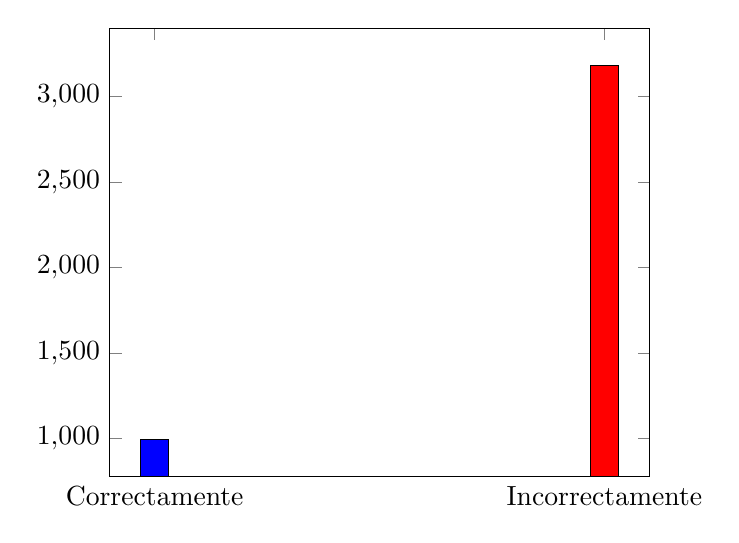
\begin{tikzpicture}
   
        \begin{axis}[
            symbolic x coords={Correctamente,Incorrectamente},
            xtick=data
          ]
          \addplot[ybar,fill=blue] coordinates {
                (Correctamente, 996)
                (Incorrectamente,3181)
            };
           \addplot[ybar,fill=red] coordinates {
              
                (Incorrectamente,3181)
            };

        \end{axis}
    \end{tikzpicture}
     \caption{Gráfico de resultados del conjunto de datos Abalone}
     
\end{figure}

%%%%%%%%%%%%%%%%%%%%%%%%
% 3. Percentage Split  %
%%%%%%%%%%%%%%%%%%%%%%%%
\subsubsection{Percentage Split}
%%%%%%%%%%%%%%%%%%%%%%%%%%%%%%%
%Sección de Percentage Split  %
%%%%%%%%%%%%%%%%%%%%%%%%%%%%%%%
d
%%%%%%%%%%%%%%%%%%%%%%%%
% 4. Supplied test set %
%%%%%%%%%%%%%%%%%%%%%%%%
\subsubsection{Supplied test set}
%%%%%%%%%%%%%%%%%%%%%%%%%%%%%%%
%Sección de Supplied test set %
%%%%%%%%%%%%%%%%%%%%%%%%%%%%%%%
e
%%%%%%%%%%%%%%%%%%%%%%%%
% 5. Conclusiones %
%%%%%%%%%%%%%%%%%%%%%%%%
\subsubsection{Conclusiones}
%%%%%%%%%%%%%%%
%Conclusiones %
%%%%%%%%%%%%%%%
Es preciso decir que para el conjunto de datos Abalone, no fue efectiva la clasificación por medio del clasificador Naïve Bayes, debido a que el porcentaje de instancias clasificadas correctamente es menor al número de instancias clasificadas incorrectamente.
%%%%%%%%%%%%%%%%%%%%%%%%
% Arboles de decisión  %
%%%%%%%%%%%%%%%%%%%%%%%%
\subsection{Arboles de decisión}
%%%%%%%%%%%%%%%%%%%%%%%%%%%%%%%
%Sección Arboles de decisión  %
%%%%%%%%%%%%%%%%%%%%%%%%%%%%%%%
f
%%%%%%%%%%%%%%%%%%%%%%%%
% 2. Cross-Validation  %
%%%%%%%%%%%%%%%%%%%%%%%%
\subsubsection{Cross-Validation}
%%%%%%%%%%%%%%%%%%%%%%%%%%%%%%%
%Sección de Cross-Validation  %
%%%%%%%%%%%%%%%%%%%%%%%%%%%%%%%
g
%%%%%%%%%%%%%%%%%%%%
% Redes neuronales %
%%%%%%%%%%%%%%%%%%%%
\subsection{Redes neuronales}
%%%%%%%%%%%%%%%%%%%%%%%%%%%%
%Sección Redes neuronales  %
%%%%%%%%%%%%%%%%%%%%%%%%%%%%
h
%%%%%%%%%%%%%%%%%%%%%%%%
% 2. Cross-Validation  %
%%%%%%%%%%%%%%%%%%%%%%%%
\subsubsection{Cross-Validation}
%%%%%%%%%%%%%%%%%%%%%%%%%%%%%%%
%Sección de Cross-Validation  %
%%%%%%%%%%%%%%%%%%%%%%%%%%%%%%%
i
%%%%%%%%%%%%%%%%
% K-Vecinos  %
%%%%%%%%%%%%%%%%
\subsection{K-Vecinos}
%%%%%%%%%%%%%%%%%%%%%%%
%Sección K-Vecinos  %
%%%%%%%%%%%%%%%%%%%%%%%
j
%%%%%%%%%%%%%%%%%%%%%%%%
% 2. Cross-Validation  %
%%%%%%%%%%%%%%%%%%%%%%%%
\subsubsection{Cross-Validation}
%%%%%%%%%%%%%%%%%%%%%%%%%%%%%%%
%Sección de Cross-Validation  %
%%%%%%%%%%%%%%%%%%%%%%%%%%%%%%%
k
%%%%%%%%%%%%%%%%%%%%%%%%%%%%%%%%%%%%
% Máquinas de vectores de soporte  %
%%%%%%%%%%%%%%%%%%%%%%%%%%%%%%%%%%%%
\subsection{Máquinas de vectores de soporte}
%%%%%%%%%%%%%%%%%%%%%%%
%Sección Máquinas de vectores de soporte  %
%%%%%%%%%%%%%%%%%%%%%%%
l
%%%%%%%%%%%%%%%%%%%%%%%%
% 2. Cross-Validation  %
%%%%%%%%%%%%%%%%%%%%%%%%
\subsubsection{Cross-Validation}
%%%%%%%%%%%%%%%%%%%%%%%%%%%%%%%
%Sección de Cross-Validation  %
%%%%%%%%%%%%%%%%%%%%%%%%%%%%%%%
m
%%%%%%%%%%%%%%%%%%%%
%    2. Rookpawn   %
%%%%%%%%%%%%%%%%%%%%
\section{Rookpawn}
%%%%%%%%%%%%%%%%%%%%%%%%%%
%Sección de  Rookpawn    %
%%%%%%%%%%%%%%%%%%%%%%%%%%
La base de datos de Rey Rook y Rey Pawn (ajedrez) fue donada por Rob Holte y generada y descrita por Alen Shapiro. La base de datos fue suministrada a Holte por Peter Clark del Instituto Turing en Glasgow.
%%%%%%%%%%%%%%%%%%%%%%%%%%%%%%%%%%%%%%%%%%%%%%%%%%%%%%%
% Atributos de abalone					        	  %
%%%%%%%%%%%%%%%%%%%%%%%%%%%%%%%%%%%%%%%%%%%%%%%%%%%%%%%
\begin{table}
\caption{Atributos de Rookpawn} % titulo de la tabla
\centering % es usado para centrar la tabla
\begin{tabular}{c c c}
% columnas centradas (3 columnas)
\hline\hline %inserts double horizontal lines
Atributo & Tipo & Dominio \\ [0.5ex]
% inserta tablas
%heading
\hline % Inserta una linea horizontal
 bkblk & Categórico & {f,t}\\ [1ex] % [1ex] Agrega un espacio vertical
 bknwy & Categórico & {f,t}\\ [1ex] % [1ex] Agrega un espacio vertical
 bkon8 & Categórico & {f,t}\\ [1ex] % [1ex] Agrega un espacio vertical
 bkona & Categórico & {f,t}\\ [1ex] % [1ex] Agrega un espacio vertical
 bkspr & Categórico & {f,t}\\ [1ex] % [1ex] Agrega un espacio vertical
 bkxbq & Categórico & {f,t}\\ [1ex] % [1ex] Agrega un espacio vertical
 bkxcr & Categórico & {f,t}\\ [1ex] % [1ex] Agrega un espacio vertical
 bkxwp & Categórico & {f,t}\\ [1ex] % [1ex] Agrega un espacio vertical
 blxwp & Categórico & {f,t}\\ [1ex] % [1ex] Agrega un espacio vertical
 bxqsq & Categórico & {f,t}\\ [1ex] % [1ex] Agrega un espacio vertical
 cntxt & Categórico & {f,t}\\ [1ex] % [1ex] Agrega un espacio vertical
 dsopp & Categórico & {f,t}\\ [1ex] % [1ex] Agrega un espacio vertical
 dwipd & Categórico & {l,g}\\ [1ex] % [1ex] Agrega un espacio vertical
 hdchk & Categórico & {f,t}\\ [1ex] % [1ex] Agrega un espacio vertical
 katri & Categórico & {n,w,b}\\ [1ex] % [1ex] Agrega un espacio vertical
 mulch & Categórico & {f,t}\\ [1ex] % [1ex] Agrega un espacio vertical
 qxmsq & Categórico & {f,t}\\ [1ex] % [1ex] Agrega un espacio vertical
 r2ar8 & Categórico & {t,f}\\ [1ex] % [1ex] Agrega un espacio vertical
 reskd & Categórico & {f,t}\\ [1ex] % [1ex] Agrega un espacio vertical
 reskr & Categórico & {f,t}\\ [1ex] % [1ex] Agrega un espacio vertical
 rimmx & Categórico & {f,t}\\ [1ex] % [1ex] Agrega un espacio vertical
 rkxwp & Categórico & {f,t}\\ [1ex] % [1ex] Agrega un espacio vertical
 rxmsq & Categórico & {f,t}\\ [1ex] % [1ex] Agrega un espacio vertical
 simpl & Categórico & {f,t}\\ [1ex] % [1ex] Agrega un espacio vertical
 skach & Categórico & {f,t}\\ [1ex] % [1ex] Agrega un espacio vertical
 skewr & Categórico & {t,f}\\ [1ex] % [1ex] Agrega un espacio vertical
 skrxp & Categórico & {f,t}\\ [1ex] % [1ex] Agrega un espacio vertical
 spcop & Categórico & {f,t}\\ [1ex] % [1ex] Agrega un espacio vertical
 stlmt & Categórico & {f,t}\\ [1ex] % [1ex] Agrega un espacio vertical
 thrsk & Categórico & {f,t}\\ [1ex] % [1ex] Agrega un espacio vertical
 wkcti & Categórico & {f,t}\\ [1ex] % [1ex] Agrega un espacio vertical
 wkna8 & Categórico & {f,t}\\ [1ex] % [1ex] Agrega un espacio vertical
 wknck & Categórico & {f,t}\\ [1ex] % [1ex] Agrega un espacio vertical
 wkovl & Categórico & {t,f}\\ [1ex] % [1ex] Agrega un espacio vertical
 wkpos & Categórico & {t,f}\\ [1ex] % [1ex] Agrega un espacio vertical
 wtoeg & Categórico & {n,t}\\ [1ex] % [1ex] Agrega un espacio vertical
 clase & Categórico & {won,nowin}\\ [1ex] % [1ex] Agrega un espacio vertical
\hline %Inserta una linea
\end{tabular}
\label{table:rookpawn} % Es usado para referise a esta tabla en el texto
\end{table}
%%%%%%%%%%%%%%%%%%%%
% Finaliza la tabla%
%%%%%%%%%%%%%%%%%%%%
%%%%%%%%%%%%%%%%%%%%%%%%%%%%%%%%%%%%%%%%%%%%%%%%%%%%%%%
% Tabla de Instancias y número de atributos %
%%%%%%%%%%%%%%%%%%%%%%%%%%%%%%%%%%%%%%%%%%%%%%%%%%%%%%%
\begin{table}
\caption{Número de Instancias y Atributos Rookpawn} % titulo de la tabla
\centering % es usado para centrar la tabla
\begin{tabular}{c c}
% columnas centradas (2 columnas)
\hline\hline %inserts double horizontal lines
Instancias & Atributos \\ [0.5ex]
% inserta tablas
%heading
\hline % Inserta una linea horizontal
3196 & 37 \\ [1ex] % [1ex] Agrega un espacio vertical
\hline %Inserta una linea
\end{tabular}
\label{table:rookpawnia} % Es usado para referise a esta tabla en el texto
\end{table}
%%%%%%%%%%%%%%%%%%%%
% Finaliza la tabla%
%%%%%%%%%%%%%%%%%%%%
%%%%%%%%%%%%%%%%
% Naïve Bayes  %
%%%%%%%%%%%%%%%%
\subsection{Naïve Bayes}
%%%%%%%%%%%%%%%%%%%%%%%
%Sección Naïve Bayes  %
%%%%%%%%%%%%%%%%%%%%%%%
%%%%%%%%%%%%%%%%%%%%%%%%
% 1. Use training set  %
%%%%%%%%%%%%%%%%%%%%%%%%
\subsubsection{Use training set}
%%%%%%%%%%%%%%%%%%%%%%%%%%%%%%%
%Sección de Use training set  %
%%%%%%%%%%%%%%%%%%%%%%%%%%%%%%%
%%%%%%%%%%%%%%%%%%%%%%%%
% 2. Cross-Validation  %
%%%%%%%%%%%%%%%%%%%%%%%%
\subsubsection{Cross-Validation}
%%%%%%%%%%%%%%%%%%%%%%%%%%%%%%%
%Sección de Cross-Validation  %
%%%%%%%%%%%%%%%%%%%%%%%%%%%%%%%
\begin{figure}[h!]
 \centering
    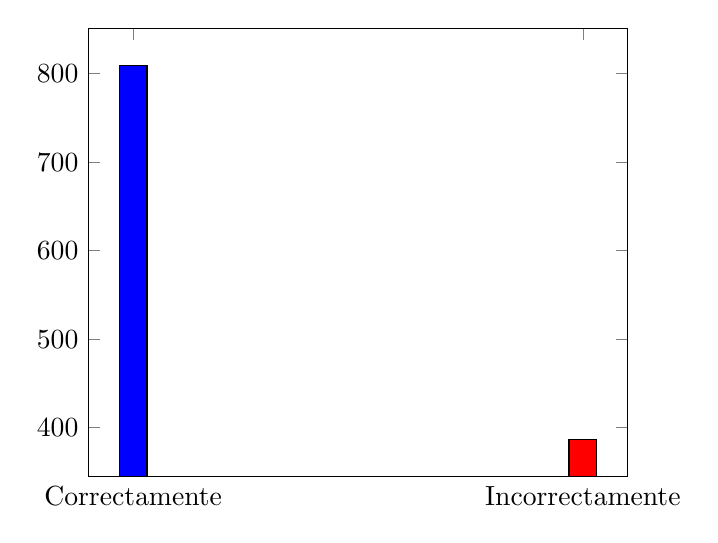
\begin{tikzpicture}
   
        \begin{axis}[
            symbolic x coords={Correctamente,Incorrectamente},
            xtick=data
          ]
          \addplot[ybar,fill=blue] coordinates {
                (Correctamente, 809)
                (Incorrectamente,387)
            };
           \addplot[ybar,fill=red] coordinates {
              
                (Incorrectamente,387)
            };

        \end{axis}
    \end{tikzpicture}
     \caption{Gráfico de resultados del conjunto de datos Rookpawn}
     
\end{figure}

%%%%%%%%%%%%%%%%%%%%%%%%
% 3. Percentage Split  %
%%%%%%%%%%%%%%%%%%%%%%%%
\subsubsection{Percentage Split}
%%%%%%%%%%%%%%%%%%%%%%%%%%%%%%%
%Sección de Percentage Split  %
%%%%%%%%%%%%%%%%%%%%%%%%%%%%%%%
%%%%%%%%%%%%%%%%%%%%%%%%
% 4. Supplied test set %
%%%%%%%%%%%%%%%%%%%%%%%%
\subsubsection{Supplied test set}
%%%%%%%%%%%%%%%%%%%%%%%%%%%%%%%
%Sección de Supplied test set %
%%%%%%%%%%%%%%%%%%%%%%%%%%%%%%%
%%%%%%%%%%%%%%%%%%%%%%%%
% 5. Conclusiones %
%%%%%%%%%%%%%%%%%%%%%%%%
\subsubsection{Conclusiones}
%%%%%%%%%%%%%%%
%Conclusiones %
%%%%%%%%%%%%%%%
Es preciso decir que para el conjunto de datos Rookpawn, fue efectiva la clasificación por medio del clasificador Naïve Bayes, debido a que el porcentaje de instancias clasificadas correctamente es mayor al número de instancias clasificadas incorrectamente.
%%%%%%%%%%%%%%%%%%%%%%%%
% Arboles de decisión  %
%%%%%%%%%%%%%%%%%%%%%%%%
\subsection{Arboles de decisión}
%%%%%%%%%%%%%%%%%%%%%%%%%%%%%%%
%Sección Arboles de decisión  %
%%%%%%%%%%%%%%%%%%%%%%%%%%%%%%%
%%%%%%%%%%%%%%%%%%%%%%%%
% 2. Cross-Validation  %
%%%%%%%%%%%%%%%%%%%%%%%%
\subsubsection{Cross-Validation}
%%%%%%%%%%%%%%%%%%%%%%%%%%%%%%%
%Sección de Cross-Validation  %
%%%%%%%%%%%%%%%%%%%%%%%%%%%%%%%
%%%%%%%%%%%%%%%%%%%%
% Redes neuronales %
%%%%%%%%%%%%%%%%%%%%
\subsection{Redes neuronales}
%%%%%%%%%%%%%%%%%%%%%%%%%%%%
%Sección Redes neuronales  %
%%%%%%%%%%%%%%%%%%%%%%%%%%%%
%%%%%%%%%%%%%%%%%%%%%%%%
% 2. Cross-Validation  %
%%%%%%%%%%%%%%%%%%%%%%%%
\subsubsection{Cross-Validation}
%%%%%%%%%%%%%%%%%%%%%%%%%%%%%%%
%Sección de Cross-Validation  %
%%%%%%%%%%%%%%%%%%%%%%%%%%%%%%%
%%%%%%%%%%%%%%%%
% K-Vecinos  %
%%%%%%%%%%%%%%%%
\subsection{K-Vecinos}
%%%%%%%%%%%%%%%%%%%%%%%
%Sección K-Vecinos  %
%%%%%%%%%%%%%%%%%%%%%%%
%%%%%%%%%%%%%%%%%%%%%%%%
% 2. Cross-Validation  %
%%%%%%%%%%%%%%%%%%%%%%%%
\subsubsection{Cross-Validation}
%%%%%%%%%%%%%%%%%%%%%%%%%%%%%%%
%Sección de Cross-Validation  %
%%%%%%%%%%%%%%%%%%%%%%%%%%%%%%%
%%%%%%%%%%%%%%%%%%%%%%%%%%%%%%%%%%%%
% Máquinas de vectores de soporte  %
%%%%%%%%%%%%%%%%%%%%%%%%%%%%%%%%%%%%
\subsection{Máquinas de vectores de soporte}
%%%%%%%%%%%%%%%%%%%%%%%
%Sección Máquinas de vectores de soporte  %
%%%%%%%%%%%%%%%%%%%%%%%
%%%%%%%%%%%%%%%%%%%%%%%%
% 2. Cross-Validation  %
%%%%%%%%%%%%%%%%%%%%%%%%
\subsubsection{Cross-Validation}
%%%%%%%%%%%%%%%%%%%%%%%%%%%%%%%
%Sección de Cross-Validation  %
%%%%%%%%%%%%%%%%%%%%%%%%%%%%%%%
%%%%%%%%%%%%%%%%%%%%%%%%%%%%%
%    3. Segmentación de Piel   %
%%%%%%%%%%%%%%%%%%%%%%%%%%%%%
\section{Segmentación de piel}
%%%%%%%%%%%%%%%%%%%%%%%%%%%%%%%%%%%%%%
%Sección de  Segmentación de Piel    %
%%%%%%%%%%%%%%%%%%%%%%%%%%%%%%%%%%%%%%
El conjunto de datos de la piel es recogida por muestreo aleatorio B, G, R valores de imágenes de caras de diferentes grupos de edad (jóvenes, de mediana y edad), grupos de raza (blanco, negro y asiático), y géneros obtenidos de la base de datos y base de datos FERET PAL . Tamaño de la muestra total de aprendizaje es 245.057; de los cuales 50.859 es las muestras de piel y 194.198 se muestras no la piel. Color FERET Image Base de datos: [Web Link], PAL Cara Base de datos del Laboratorio de Envejecimiento Productivo, de la Universidad de Texas en Dallas
%%%%%%%%%%%%%%%%%%%%%%%%%%%%%%%%%%%%%%%%%%%%%%%%%%%%%%%
% Tabla de Instancias y número de atributos %
%%%%%%%%%%%%%%%%%%%%%%%%%%%%%%%%%%%%%%%%%%%%%%%%%%%%%%%
\begin{table}
\caption{Número de Instancias y Atributos Segmentación de piel} % titulo de la tabla
\centering % es usado para centrar la tabla
\begin{tabular}{c c}
% columnas centradas (2 columnas)
\hline\hline %inserts double horizontal lines
Instancias & Atributos \\ [0.5ex]
% inserta tablas
%heading
\hline % Inserta una linea horizontal
245057 & 4 \\ [1ex] % [1ex] Agrega un espacio vertical
\hline %Inserta una linea
\end{tabular}
\label{table:segmentacionpielia} % Es usado para referise a esta tabla en el texto
\end{table}
%%%%%%%%%%%%%%%%%%%%
% Finaliza la tabla%
%%%%%%%%%%%%%%%%%%%%
%%%%%%%%%%%%%%%%%%%%%%%%%%%%%%%%%%%%%%%%%%%%%%%%%%%%%%%
% Atributos de segmentacion piel       	              %
%%%%%%%%%%%%%%%%%%%%%%%%%%%%%%%%%%%%%%%%%%%%%%%%%%%%%%%
\begin{table}
\caption{Atributos de Segmentación de piel} % titulo de la tabla
\centering % es usado para centrar la tabla
\begin{tabular}{c c c}
% columnas centradas (3 columnas)
\hline\hline %inserts double horizontal lines
Atributo & Tipo & Dominio \\ [0.5ex]
% inserta tablas
%heading
\hline % Inserta una linea horizontal
R & Entero & 0,..255\\ [1ex] % [1ex] Agrega un espacio vertical
G & Entero & 0,..255\\ [1ex] % [1ex] Agrega un espacio vertical
B & Entero & 0,..255\\ [1ex] % [1ex] Agrega un espacio vertical
Clase & Categórico & {1,2}\\ [1ex] % [1ex] Agrega un espacio vertical
\hline %Inserta una linea
\end{tabular}
\label{table:segmentacionpiela} % Es usado para referise a esta tabla en el texto
\end{table}
%%%%%%%%%%%%%%%%%%%%
% Finaliza la tabla%
%%%%%%%%%%%%%%%%%%%%

%%%%%%%%%%%%%%%%
% Naïve Bayes  %
%%%%%%%%%%%%%%%%
\subsection{Naïve Bayes}
%%%%%%%%%%%%%%%%%%%%%%%
%Sección Naïve Bayes  %
%%%%%%%%%%%%%%%%%%%%%%%
%%%%%%%%%%%%%%%%%%%%%%%%
% 1. Use training set  %
%%%%%%%%%%%%%%%%%%%%%%%%
\subsubsection{Use training set}
%%%%%%%%%%%%%%%%%%%%%%%%%%%%%%%
%Sección de Use training set  %
%%%%%%%%%%%%%%%%%%%%%%%%%%%%%%%
%%%%%%%%%%%%%%%%%%%%%%%%
% 2. Cross-Validation  %
%%%%%%%%%%%%%%%%%%%%%%%%
\subsubsection{Cross-Validation}
%%%%%%%%%%%%%%%%%%%%%%%%%%%%%%%
%Sección de Cross-Validation  %
%%%%%%%%%%%%%%%%%%%%%%%%%%%%%%%
%%%%%%%%%%%%%%%%%%%%%%%%
% 3. Percentage Split  %
%%%%%%%%%%%%%%%%%%%%%%%%
\subsubsection{Percentage Split}
%%%%%%%%%%%%%%%%%%%%%%%%%%%%%%%
%Sección de Percentage Split  %
%%%%%%%%%%%%%%%%%%%%%%%%%%%%%%%
%%%%%%%%%%%%%%%%%%%%%%%%
% 4. Supplied test set %
%%%%%%%%%%%%%%%%%%%%%%%%
\subsubsection{Supplied test set}
%%%%%%%%%%%%%%%%%%%%%%%%%%%%%%%
%Sección de Supplied test set %
%%%%%%%%%%%%%%%%%%%%%%%%%%%%%%%
%%%%%%%%%%%%%%%%%%%%%%%%
% 5. Conclusiones %
%%%%%%%%%%%%%%%%%%%%%%%%
\subsubsection{Conclusiones}
%%%%%%%%%%%%%%%
%Conclusiones %
%%%%%%%%%%%%%%%
Es preciso decir que para el conjunto de datos Segmentación de Piel, fue efectiva la clasificación por medio del clasificador Naïve Bayes, debido a que el porcentaje de instancias clasificadas correctamente es mayor al número de instancias clasificadas incorrectamente.
%%%%%%%%%%%%%%%%%%%%%%%%
% Arboles de decisión  %
%%%%%%%%%%%%%%%%%%%%%%%%
\subsection{Arboles de decisión}
%%%%%%%%%%%%%%%%%%%%%%%%%%%%%%%
%Sección Arboles de decisión  %
%%%%%%%%%%%%%%%%%%%%%%%%%%%%%%%
%%%%%%%%%%%%%%%%%%%%%%%%
% 2. Cross-Validation  %
%%%%%%%%%%%%%%%%%%%%%%%%
\subsubsection{Cross-Validation}
%%%%%%%%%%%%%%%%%%%%%%%%%%%%%%%
%Sección de Cross-Validation  %
%%%%%%%%%%%%%%%%%%%%%%%%%%%%%%%
\begin{figure}[h!]
 \centering
    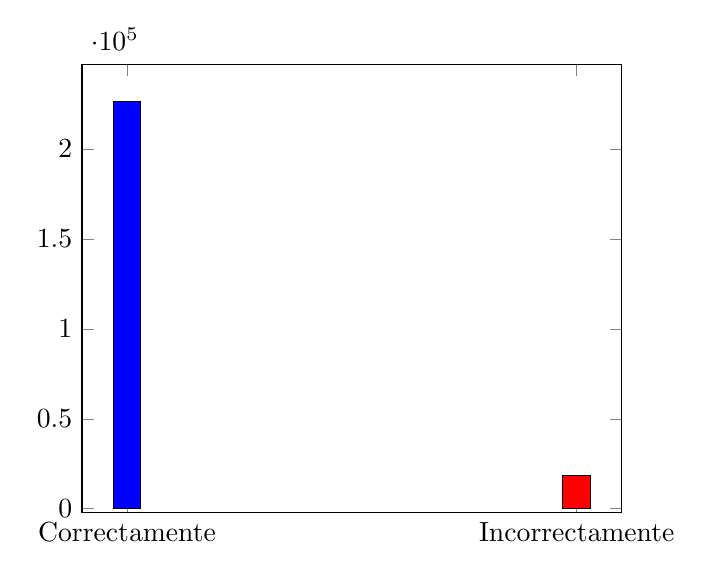
\begin{tikzpicture}
   
        \begin{axis}[
            symbolic x coords={Correctamente,Incorrectamente},
            xtick=data
          ]
          \addplot[ybar,fill=blue] coordinates {
                (Correctamente, 226407)
                (Incorrectamente,18650)
            };
           \addplot[ybar,fill=red] coordinates {
              
                (Incorrectamente,18650)
            };

        \end{axis}
    \end{tikzpicture}
     \caption{Gráfico de resultados del conjunto de datos Segmentación de piel}
     
\end{figure}
%%%%%%%%%%%%%%%%%%%%
% Redes neuronales %
%%%%%%%%%%%%%%%%%%%%
\subsection{Redes neuronales}
%%%%%%%%%%%%%%%%%%%%%%%%%%%%
%Sección Redes neuronales  %
%%%%%%%%%%%%%%%%%%%%%%%%%%%%
%%%%%%%%%%%%%%%%%%%%%%%%
% 2. Cross-Validation  %
%%%%%%%%%%%%%%%%%%%%%%%%
\subsubsection{Cross-Validation}
%%%%%%%%%%%%%%%%%%%%%%%%%%%%%%%
%Sección de Cross-Validation  %
%%%%%%%%%%%%%%%%%%%%%%%%%%%%%%%
%%%%%%%%%%%%%%%%
% K-Vecinos  %
%%%%%%%%%%%%%%%%
\subsection{K-Vecinos}
%%%%%%%%%%%%%%%%%%%%%%%
%Sección K-Vecinos  %
%%%%%%%%%%%%%%%%%%%%%%%
%%%%%%%%%%%%%%%%%%%%%%%%
% 2. Cross-Validation  %
%%%%%%%%%%%%%%%%%%%%%%%%
\subsubsection{Cross-Validation}
%%%%%%%%%%%%%%%%%%%%%%%%%%%%%%%
%Sección de Cross-Validation  %
%%%%%%%%%%%%%%%%%%%%%%%%%%%%%%%
%%%%%%%%%%%%%%%%%%%%%%%%%%%%%%%%%%%%
% Máquinas de vectores de soporte  %
%%%%%%%%%%%%%%%%%%%%%%%%%%%%%%%%%%%%
\subsection{Máquinas de vectores de soporte}
%%%%%%%%%%%%%%%%%%%%%%%
%Sección Máquinas de vectores de soporte  %
%%%%%%%%%%%%%%%%%%%%%%%
%%%%%%%%%%%%%%%%%%%%%%%%
% 2. Cross-Validation  %
%%%%%%%%%%%%%%%%%%%%%%%%
\subsubsection{Cross-Validation}
%%%%%%%%%%%%%%%%%%%%%%%%%%%%%%%
%Sección de Cross-Validation  %
%%%%%%%%%%%%%%%%%%%%%%%%%%%%%%%
%%%%%%%%%%%%%%%%%%%%%%%%%%%%%
%    4. Pokerhand   %
%%%%%%%%%%%%%%%%%%%%%%%%%%%%%
\section{Pokerhand}
%%%%%%%%%%%%%%%%%%%%%%%%%%%%%%%%%%%%%%
%Sección de Pokerhand    %
%%%%%%%%%%%%%%%%%%%%%%%%%%%%%%%%%%%%%%
Cada registro es un ejemplo de una mano con cinco cartas procedentes de una baraja de 52. Cada carta se describe el uso de dos atributos (traje y de la fila), para un total de 10 atributos de predicción. Hay un atributo de clase que describe el "Poker Hand". El orden de las cartas es importante, por lo que hay 480 posibles manos Royal Flush.
%%%%%%%%%%%%%%%%%%%%%%%%%%%%%%%%%%%%%%%%%%%%%%%%%%%%%%%
% Tabla de Instancias y número de atributos %
%%%%%%%%%%%%%%%%%%%%%%%%%%%%%%%%%%%%%%%%%%%%%%%%%%%%%%%
\begin{table}
\caption{Número de Instancias y Atributos Pokerhand} % titulo de la tabla
\centering % es usado para centrar la tabla
\begin{tabular}{c c}
% columnas centradas (2 columnas)
\hline\hline %inserts double horizontal lines
Instancias & Atributos \\ [0.5ex]
% inserta tablas
%heading
\hline % Inserta una linea horizontal
25010 & 11 \\ [1ex] % [1ex] Agrega un espacio vertical
\hline %Inserta una linea
\end{tabular}
\label{table:pokerhandia} % Es usado para referise a esta tabla en el texto
\end{table}
%%%%%%%%%%%%%%%%%%%%
% Finaliza la tabla%
%%%%%%%%%%%%%%%%%%%%
%%%%%%%%%%%%%%%%%%%%%%%%%%%%%%%%%%%%%%%%%%%%%%%%%%%%%%%
% Atributos de pokerhand            	              %
%%%%%%%%%%%%%%%%%%%%%%%%%%%%%%%%%%%%%%%%%%%%%%%%%%%%%%%
\begin{table}
\caption{Atributos de Pokerhand} % titulo de la tabla
\centering % es usado para centrar la tabla
\begin{tabular}{c c c}
% columnas centradas (3 columnas)
\hline\hline %inserts double horizontal lines
Atributo & Tipo & Dominio \\ [0.5ex]
% inserta tablas
%heading
\hline % Inserta una linea horizontal
juegocarta1 & real &  1,..4\\ [1ex] % [1ex] Agrega un espacio vertical
posicioncarta1 & real & 1,..13\\ [1ex] % [1ex] Agrega un espacio vertical
juegocarta2 & real & 1,..4\\ [1ex] % [1ex] Agrega un espacio vertical
posicioncarta2 & real & 1,..13\\ [1ex] % [1ex] Agrega un espacio vertical
juegocarta3 & real & 1,..4\\ [1ex] % [1ex] Agrega un espacio vertical
posicioncarta3 & real & 1,..13\\ [1ex] % [1ex] Agrega un espacio vertical
juegocarta4 & real & 1,..4\\ [1ex] % [1ex] Agrega un espacio vertical
posicioncarta4 & real & 1,..13\\ [1ex] % [1ex] Agrega un espacio vertical
juegocarta5 & real& 1,..4\\ [1ex] % [1ex] Agrega un espacio vertical
posicioncarta5 & real & 1,..13\\ [1ex] % [1ex] Agrega un espacio vertical
clase & Categórico & 0,..9\\ [1ex] % [1ex] Agrega un espacio vertical
\hline %Inserta una linea
\end{tabular}
\label{table:pokerhanda} % Es usado para referise a esta tabla en el texto
\end{table}
%%%%%%%%%%%%%%%%%%%%
% Finaliza la tabla%
%%%%%%%%%%%%%%%%%%%%
%%%%%%%%%%%%%%%%
% Naïve Bayes  %
%%%%%%%%%%%%%%%%
\subsection{Naïve Bayes}
%%%%%%%%%%%%%%%%%%%%%%%
%Sección Naïve Bayes  %
%%%%%%%%%%%%%%%%%%%%%%%
%%%%%%%%%%%%%%%%%%%%%%%%
% 1. Use training set  %
%%%%%%%%%%%%%%%%%%%%%%%%
\subsubsection{Use training set}
%%%%%%%%%%%%%%%%%%%%%%%%%%%%%%%
%Sección de Use training set  %
%%%%%%%%%%%%%%%%%%%%%%%%%%%%%%%
%%%%%%%%%%%%%%%%%%%%%%%%
% 2. Cross-Validation  %
%%%%%%%%%%%%%%%%%%%%%%%%
\subsubsection{Cross-Validation}
%%%%%%%%%%%%%%%%%%%%%%%%%%%%%%%
%Sección de Cross-Validation  %
%%%%%%%%%%%%%%%%%%%%%%%%%%%%%%%
\begin{figure}[h!]
 \centering
    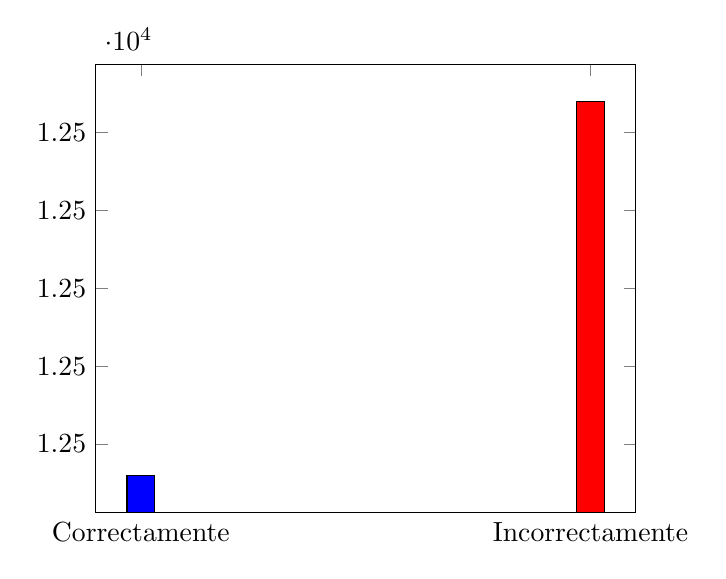
\begin{tikzpicture}
   
        \begin{axis}[
            symbolic x coords={Correctamente,Incorrectamente},
            xtick=data
          ]
          \addplot[ybar,fill=blue] coordinates {
                (Correctamente, 12493)
                (Incorrectamente,12517)
            };
           \addplot[ybar,fill=red] coordinates {
              
                (Incorrectamente,12517)
            };

        \end{axis}
    \end{tikzpicture}
     \caption{Gráfico de resultados del conjunto de datos Pokerhand}
     
\end{figure}
%%%%%%%%%%%%%%%%%%%%%%%%
% 3. Percentage Split  %
%%%%%%%%%%%%%%%%%%%%%%%%
\subsubsection{Percentage Split}
%%%%%%%%%%%%%%%%%%%%%%%%%%%%%%%
%Sección de Percentage Split  %
%%%%%%%%%%%%%%%%%%%%%%%%%%%%%%%
%%%%%%%%%%%%%%%%%%%%%%%%
% 4. Supplied test set %
%%%%%%%%%%%%%%%%%%%%%%%%
\subsubsection{Supplied test set}
%%%%%%%%%%%%%%%%%%%%%%%%%%%%%%%
%Sección de Supplied test set %
%%%%%%%%%%%%%%%%%%%%%%%%%%%%%%%
%%%%%%%%%%%%%%%%%%%%%%%%
% 5. Conclusiones %
%%%%%%%%%%%%%%%%%%%%%%%%
\subsubsection{Conclusiones}
%%%%%%%%%%%%%%%
%Conclusiones %
%%%%%%%%%%%%%%%
Es preciso decir que para el conjunto de datos Pokerhand, no fue efectiva la clasificación por medio del clasificador Naïve Bayes, debido a que el porcentaje de instancias clasificadas correctamente es similar al número de instancias clasificadas incorrectamente.
%%%%%%%%%%%%%%%%%%%%%%%%
% Arboles de decisión  %
%%%%%%%%%%%%%%%%%%%%%%%%
\subsection{Arboles de decisión}
%%%%%%%%%%%%%%%%%%%%%%%%%%%%%%%
%Sección Arboles de decisión  %
%%%%%%%%%%%%%%%%%%%%%%%%%%%%%%%
%%%%%%%%%%%%%%%%%%%%%%%%
% 2. Cross-Validation  %
%%%%%%%%%%%%%%%%%%%%%%%%
\subsubsection{Cross-Validation}
%%%%%%%%%%%%%%%%%%%%%%%%%%%%%%%
%Sección de Cross-Validation  %
%%%%%%%%%%%%%%%%%%%%%%%%%%%%%%%
%%%%%%%%%%%%%%%%%%%%
% Redes neuronales %
%%%%%%%%%%%%%%%%%%%%
\subsection{Redes neuronales}
%%%%%%%%%%%%%%%%%%%%%%%%%%%%
%Sección Redes neuronales  %
%%%%%%%%%%%%%%%%%%%%%%%%%%%%
%%%%%%%%%%%%%%%%%%%%%%%%
% 2. Cross-Validation  %
%%%%%%%%%%%%%%%%%%%%%%%%
\subsubsection{Cross-Validation}
%%%%%%%%%%%%%%%%%%%%%%%%%%%%%%%
%Sección de Cross-Validation  %
%%%%%%%%%%%%%%%%%%%%%%%%%%%%%%%
%%%%%%%%%%%%%%%%
% K-Vecinos  %
%%%%%%%%%%%%%%%%
\subsection{K-Vecinos}
%%%%%%%%%%%%%%%%%%%%%%%
%Sección K-Vecinos  %
%%%%%%%%%%%%%%%%%%%%%%%
%%%%%%%%%%%%%%%%%%%%%%%%
% 2. Cross-Validation  %
%%%%%%%%%%%%%%%%%%%%%%%%
\subsubsection{Cross-Validation}
%%%%%%%%%%%%%%%%%%%%%%%%%%%%%%%
%Sección de Cross-Validation  %
%%%%%%%%%%%%%%%%%%%%%%%%%%%%%%%
%%%%%%%%%%%%%%%%%%%%%%%%%%%%%%%%%%%%
% Máquinas de vectores de soporte  %
%%%%%%%%%%%%%%%%%%%%%%%%%%%%%%%%%%%%
\subsection{Máquinas de vectores de soporte}
%%%%%%%%%%%%%%%%%%%%%%%
%Sección Máquinas de vectores de soporte  %
%%%%%%%%%%%%%%%%%%%%%%%
%%%%%%%%%%%%%%%%%%%%%%%%
% 2. Cross-Validation  %
%%%%%%%%%%%%%%%%%%%%%%%%
\subsubsection{Cross-Validation}
%%%%%%%%%%%%%%%%%%%%%%%%%%%%%%%
%Sección de Cross-Validation  %
%%%%%%%%%%%%%%%%%%%%%%%%%%%%%%%
%%%%%%%%%%%%%%%%%%%%%%%%%%%%%
%    5. Tic-tac-toe   %
%%%%%%%%%%%%%%%%%%%%%%%%%%%%%
\section{Tic-tac-toe}
%%%%%%%%%%%%%%%%%%%%%%%%%%%%%%%%%%%%%%
%Sección de Tic-tac-toe    %
%%%%%%%%%%%%%%%%%%%%%%%%%%%%%%%%%%%%%%
La base de datos "Tic-Tac-Toe Endgame" consta de 9 atributos, 958 instancias, y fue aplicada para el área de los juegos. Fue donada el 19 de agosto del año de 1991 por David W. Aha.
El contenido de ésta base de datos es todas las posibles configuraciones del tablero al final de un juego de tic-tac-toe (tres en raya en español), donde "x" es el que ha jugado primero. El objetivo es "victoria para x" (por ejemplo, verdadero cuando "x" tiene una de 8 posibles formas de crear un "tres en raya").
%%%%%%%%%%%%%%%%%%%%%%%%%%%%%%%%%%%%%%%%%%%%%%%%%%%%%%%
% Tabla de Instancias y número de atributos %
%%%%%%%%%%%%%%%%%%%%%%%%%%%%%%%%%%%%%%%%%%%%%%%%%%%%%%%
\begin{table}
\caption{Número de Instancias y Atributos Tic-tac-toe} % titulo de la tabla
\centering % es usado para centrar la tabla
\begin{tabular}{c c}
% columnas centradas (2 columnas)
\hline\hline %inserts double horizontal lines
Instancias & Atributos \\ [0.5ex]
% inserta tablas
%heading
\hline % Inserta una linea horizontal
958 & 10 \\ [1ex] % [1ex] Agrega un espacio vertical
\hline %Inserta una linea
\end{tabular}
\label{table:tictactoeia} % Es usado para referise a esta tabla en el texto
\end{table}
%%%%%%%%%%%%%%%%%%%%
% Finaliza la tabla%
%%%%%%%%%%%%%%%%%%%%

%%%%%%%%%%%%%%%%%%%%%%%%%%%%%%%%%%%%%%%%%%%%%%%%%%%%%%%
% Atributos de tictactoe            	              %
%%%%%%%%%%%%%%%%%%%%%%%%%%%%%%%%%%%%%%%%%%%%%%%%%%%%%%%
\begin{table}
\caption{Atributos de Tic tac toe} % titulo de la tabla
\centering % es usado para centrar la tabla
\begin{tabular}{c c c}
% columnas centradas (3 columnas)
\hline\hline %inserts double horizontal lines
Atributo & Tipo & Dominio \\ [0.5ex]
% inserta tablas
%heading
\hline % Inserta una linea horizontal
cuadroSuperiorIzq	& Categórico & {x,o,b}\\ [1ex] % [1ex] Agrega un espacio vertical
cuadroMedioSup	& Categórico & {x,o,b}\\ [1ex] % [1ex] Agrega un espacio vertical
cuadroDerechoSup	& Categórico & {x,o,b}\\ [1ex] % [1ex] Agrega un espacio vertical
cuadroMedioSup	& Categórico & {x,o,b}\\ [1ex] % [1ex] Agrega un espacio vertical
cuadroMedioMedio	& Categórico & {x,o,b}\\ [1ex] % [1ex] Agrega un espacio vertical
cuadroMedioDer	& Categórico & {x,o,b}\\ [1ex] % [1ex] Agrega un espacio vertical
cuadroInfIzq	& Categórico & {x,o,b}\\ [1ex] % [1ex] Agrega un espacio vertical
cuadroInfMedio	& Categórico & {x,o,b}\\ [1ex] % [1ex] Agrega un espacio vertical
cuadroInfDer	& Categórico & {x,o,b}\\ [1ex] % [1ex] Agrega un espacio vertical
clase	& Categórico & {positive,negative}\\ [1ex] % [1ex] Agrega un espacio vertical
\hline %Inserta una linea
\end{tabular}
\label{table:tictactoea} % Es usado para referise a esta tabla en el texto
\end{table}
%%%%%%%%%%%%%%%%%%%%
% Finaliza la tabla%
%%%%%%%%%%%%%%%%%%%%
%%%%%%%%%%%%%%%%
% Naïve Bayes  %
%%%%%%%%%%%%%%%%
\subsection{Naïve Bayes}
%%%%%%%%%%%%%%%%%%%%%%%
%Sección Naïve Bayes  %
%%%%%%%%%%%%%%%%%%%%%%%
%%%%%%%%%%%%%%%%%%%%%%%%
% 1. Use training set  %
%%%%%%%%%%%%%%%%%%%%%%%%
\subsubsection{Use training set}
%%%%%%%%%%%%%%%%%%%%%%%%%%%%%%%
%Sección de Use training set  %
%%%%%%%%%%%%%%%%%%%%%%%%%%%%%%%
%%%%%%%%%%%%%%%%%%%%%%%%
% 2. Cross-Validation  %
%%%%%%%%%%%%%%%%%%%%%%%%
\subsubsection{Cross-Validation}
%%%%%%%%%%%%%%%%%%%%%%%%%%%%%%%
%Sección de Cross-Validation  %
%%%%%%%%%%%%%%%%%%%%%%%%%%%%%%%
\begin{figure}[h!]
 \centering
    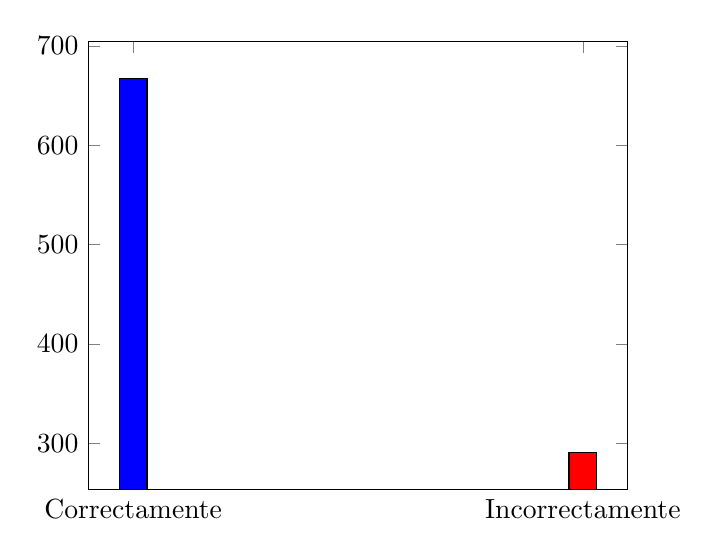
\begin{tikzpicture}
   
        \begin{axis}[
            symbolic x coords={Correctamente,Incorrectamente},
            xtick=data
          ]
          \addplot[ybar,fill=blue] coordinates {
                (Correctamente, 667)
                (Incorrectamente,291)
            };
           \addplot[ybar,fill=red] coordinates {
              
                (Incorrectamente,291)
            };

        \end{axis}
    \end{tikzpicture}
     \caption{Gráfico de resultados del conjunto de datos Tic tac toe}
     
\end{figure}
%%%%%%%%%%%%%%%%%%%%%%%%
% 3. Percentage Split  %
%%%%%%%%%%%%%%%%%%%%%%%%
\subsubsection{Percentage Split}
%%%%%%%%%%%%%%%%%%%%%%%%%%%%%%%
%Sección de Percentage Split  %
%%%%%%%%%%%%%%%%%%%%%%%%%%%%%%%
%%%%%%%%%%%%%%%%%%%%%%%%
% 4. Supplied test set %
%%%%%%%%%%%%%%%%%%%%%%%%
\subsubsection{Supplied test set}
%%%%%%%%%%%%%%%%%%%%%%%%%%%%%%%
%Sección de Supplied test set %
%%%%%%%%%%%%%%%%%%%%%%%%%%%%%%%
%%%%%%%%%%%%%%%%%%%%%%%%
% 5. Conclusiones %
%%%%%%%%%%%%%%%%%%%%%%%%
\subsubsection{Conclusiones}
%%%%%%%%%%%%%%%
%Conclusiones %
%%%%%%%%%%%%%%%
Es preciso decir que para el conjunto de datos Tic-tac-toe, fue efectiva la clasificación por medio del clasificador Naïve Bayes, debido a que el porcentaje de instancias clasificadas correctamente es mayor al número de instancias clasificadas incorrectamente.
%%%%%%%%%%%%%%%%%%%%%%%%
% Arboles de decisión  %
%%%%%%%%%%%%%%%%%%%%%%%%
\subsection{Arboles de decisión}
%%%%%%%%%%%%%%%%%%%%%%%%%%%%%%%
%Sección Arboles de decisión  %
%%%%%%%%%%%%%%%%%%%%%%%%%%%%%%%
%%%%%%%%%%%%%%%%%%%%%%%%
% 2. Cross-Validation  %
%%%%%%%%%%%%%%%%%%%%%%%%
\subsubsection{Cross-Validation}
%%%%%%%%%%%%%%%%%%%%%%%%%%%%%%%
%Sección de Cross-Validation  %
%%%%%%%%%%%%%%%%%%%%%%%%%%%%%%%
%%%%%%%%%%%%%%%%%%%%
% Redes neuronales %
%%%%%%%%%%%%%%%%%%%%
\subsection{Redes neuronales}
%%%%%%%%%%%%%%%%%%%%%%%%%%%%
%Sección Redes neuronales  %
%%%%%%%%%%%%%%%%%%%%%%%%%%%%
%%%%%%%%%%%%%%%%%%%%%%%%
% 2. Cross-Validation  %
%%%%%%%%%%%%%%%%%%%%%%%%
\subsubsection{Cross-Validation}
%%%%%%%%%%%%%%%%%%%%%%%%%%%%%%%
%Sección de Cross-Validation  %
%%%%%%%%%%%%%%%%%%%%%%%%%%%%%%%
%%%%%%%%%%%%%%%%
% K-Vecinos  %
%%%%%%%%%%%%%%%%
\subsection{K-Vecinos}
%%%%%%%%%%%%%%%%%%%%%%%
%Sección K-Vecinos  %
%%%%%%%%%%%%%%%%%%%%%%%
%%%%%%%%%%%%%%%%%%%%%%%%
% 2. Cross-Validation  %
%%%%%%%%%%%%%%%%%%%%%%%%
\subsubsection{Cross-Validation}
%%%%%%%%%%%%%%%%%%%%%%%%%%%%%%%
%Sección de Cross-Validation  %
%%%%%%%%%%%%%%%%%%%%%%%%%%%%%%%
%%%%%%%%%%%%%%%%%%%%%%%%%%%%%%%%%%%%
% Máquinas de vectores de soporte  %
%%%%%%%%%%%%%%%%%%%%%%%%%%%%%%%%%%%%
\subsection{Máquinas de vectores de soporte}
%%%%%%%%%%%%%%%%%%%%%%%
%Sección Máquinas de vectores de soporte  %
%%%%%%%%%%%%%%%%%%%%%%%
%%%%%%%%%%%%%%%%%%%%%%%%
% 2. Cross-Validation  %
%%%%%%%%%%%%%%%%%%%%%%%%
\subsubsection{Cross-Validation}
%%%%%%%%%%%%%%%%%%%%%%%%%%%%%%%
%Sección de Cross-Validation  %
%%%%%%%%%%%%%%%%%%%%%%%%%%%%%%%
%%%%%%%%%%%%%%%%%%%%%%%%%%%%%
%    6. Seismic-bump   %
%%%%%%%%%%%%%%%%%%%%%%%%%%%%%
\section{Seismic-bump}
%%%%%%%%%%%%%%%%%%%%%%%%%%%%%%%%%%%%%%
%Sección de Seismic-bump    %
%%%%%%%%%%%%%%%%%%%%%%%%%%%%%%%%%%%%%%
La complejidad  de los procesos sísmicos y gran desproporción entre el número de eventos sísmicos de baja energía y el número de fenómenos de alta energía hace que las técnicas estadísticas son insuficientes para predecir la peligrosidad sísmica . Por lo tanto , es esencial para la búsqueda de nuevas oportunidades de una mejor predicción de peligros, también utilizando métodos de aprendizaje automático . En las técnicas de agrupamiento de datos de evaluación de la peligrosidad sísmica se puede aplicar ( Lesniak A. , Isakow Z. : . . Clustering El espacio-tiempo de los eventos sísmicos y evaluación hzard en la mina de carbón Zabrze - Bielszowice , Polonia Int. Journal of Rock Mechanics y Ciencias de la Minería , de 46 (5), 2009 , 918-928) , y para la predicción de temblores sísmicos redes neuronales artificiales se utilizan ( Kabiesz , J. : . Efecto de la forma de los datos sobre la calidad de la mina de la previsión de riesgos temblores usando redes neuronales geotécnica y geológica Ingeniería, 24 (5), 2005, 1131-1147).En la mayoría de las aplicaciones, los resultados obtenidos por los métodos mencionados se presentan en forma de dos estados que se interpretan como « peligrosos y « no peligrosos.Distribución desequilibrada de positivo ("estado peligroso") y negativo ("estado no peligrosos") ejemplos es un problema grave en la predicción del riesgo sísmico. Actualmente se utilizan métodos son todavía insuficientes para lograr una buena sensibilidad y especificidad de las predicciones. Los datos presentados conjunto se caracterizan por una distribución desequilibrada de los ejemplos positivos y negativos. 
En el conjunto de datos no están a sólo 170 ejemplos positivos que representan la clase 1.
%%%%%%%%%%%%%%%%%%%%%%%%%%%%%%%%%%%%%%%%%%%%%%%%%%%%%%%
% Tabla de Instancias y número de atributos %
%%%%%%%%%%%%%%%%%%%%%%%%%%%%%%%%%%%%%%%%%%%%%%%%%%%%%%%
\begin{table}
\caption{Número de Instancias y Atributos de Seismic bump} % titulo de la tabla
\centering % es usado para centrar la tabla
\begin{tabular}{c c}
% columnas centradas (2 columnas)
\hline\hline %inserts double horizontal lines
Instancias & Atributos \\ [0.5ex]
% inserta tablas
%heading
\hline % Inserta una linea horizontal
2584 & 19 \\ [1ex] % [1ex] Agrega un espacio vertical
\hline %Inserta una linea
\end{tabular}
\label{table:seismicbumpia} % Es usado para referise a esta tabla en el texto
\end{table}
%%%%%%%%%%%%%%%%%%%%
% Finaliza la tabla%
%%%%%%%%%%%%%%%%%%%%

%%%%%%%%%%%%%%%%%%%%%%%%%%%%%%%%%%%%%%%%%%%%%%%%%%%%%%%
% Atributos de Seismicbump            	              %
%%%%%%%%%%%%%%%%%%%%%%%%%%%%%%%%%%%%%%%%%%%%%%%%%%%%%%%
\begin{table}
\caption{Atributos de Seismicbump} % titulo de la tabla
\centering % es usado para centrar la tabla
\begin{tabular}{c c c}
% columnas centradas (3 columnas)
\hline\hline %inserts double horizontal lines
Atributo & Tipo & Dominio \\ [0.5ex]
% inserta tablas
%heading
\hline % Inserta una linea horizontal
Sísmico	& Categórico	& {a,b,c,d}\\ [1ex] % [1ex] Agrega un espacio vertical
Sísmicoacustico	& Categórico	& {a,b,c,d}\\ [1ex] % [1ex] Agrega un espacio vertical
Cambio	& Categórico	& {W, N}\\ [1ex] % [1ex] Agrega un espacio vertical
Genergia	& Real	& 48,72,-30,448,400,…\\ [1ex] % [1ex] Agrega un espacio vertical
Pulsosg	& Real	& 48,72,-30,448,400,…\\ [1ex] % [1ex] Agrega un espacio vertical
Peligrog	& Categórico	& {a,b,c,d}\\ [1ex] % [1ex] Agrega un espacio vertical
Ngolpes	& Real	& 48,72,-30,448,400,…\\ [1ex] % [1ex] Agrega un espacio vertical
Ngolpes2	& Real	& 48,72,-30,448,400,…\\ [1ex] % [1ex] Agrega un espacio vertical
Ngolpes3	& Real	& 48,72,-30,448,400,…\\ [1ex] % [1ex] Agrega un espacio vertical
Ngolpes4	& Real	& 48,72,-30,448,400,…\\ [1ex] % [1ex] Agrega un espacio vertical
Ngolpes5	& Real	& 48,72,-30,448,400,…\\ [1ex] % [1ex] Agrega un espacio vertical
Ngolpes6	& Real & 48,72,-30,448,400,…\\ [1ex] % [1ex] Agrega un espacio vertical
Ngolpes7	& Real	& 48,72,-30,448,400,…\\ [1ex] % [1ex] Agrega un espacio vertical
Ngolpes89	& Real	& 48,72,-30,448,400,…\\ [1ex] % [1ex] Agrega un espacio vertical
Energía	& Real	& 48,72,-30,448,400,…\\ [1ex] % [1ex] Agrega un espacio vertical
Maxenergia& 	Real	& 48,72,-30,448,400,…\\ [1ex] % [1ex] Agrega un espacio vertical
Clases	&  Categórico	& {1,0}\\ [1ex] % [1ex] Agrega un espacio vertical
\hline %Inserta una linea
\end{tabular}
\label{table:seismicbumpa} % Es usado para referise a esta tabla en el texto
\end{table}
%%%%%%%%%%%%%%%%%%%%
% Finaliza la tabla%
%%%%%%%%%%%%%%%%%%%%
%%%%%%%%%%%%%%%%
% Naïve Bayes  %
%%%%%%%%%%%%%%%%
\subsection{Naïve Bayes}
%%%%%%%%%%%%%%%%%%%%%%%
%Sección Naïve Bayes  %
%%%%%%%%%%%%%%%%%%%%%%%
%%%%%%%%%%%%%%%%%%%%%%%%
% 1. Use training set  %
%%%%%%%%%%%%%%%%%%%%%%%%
\subsubsection{Use training set}
%%%%%%%%%%%%%%%%%%%%%%%%%%%%%%%
%Sección de Use training set  %
%%%%%%%%%%%%%%%%%%%%%%%%%%%%%%%
%%%%%%%%%%%%%%%%%%%%%%%%
% 2. Cross-Validation  %
%%%%%%%%%%%%%%%%%%%%%%%%
\subsubsection{Cross-Validation}
%%%%%%%%%%%%%%%%%%%%%%%%%%%%%%%
%Sección de Cross-Validation  %
%%%%%%%%%%%%%%%%%%%%%%%%%%%%%%%
\begin{figure}[h!]
 \centering
    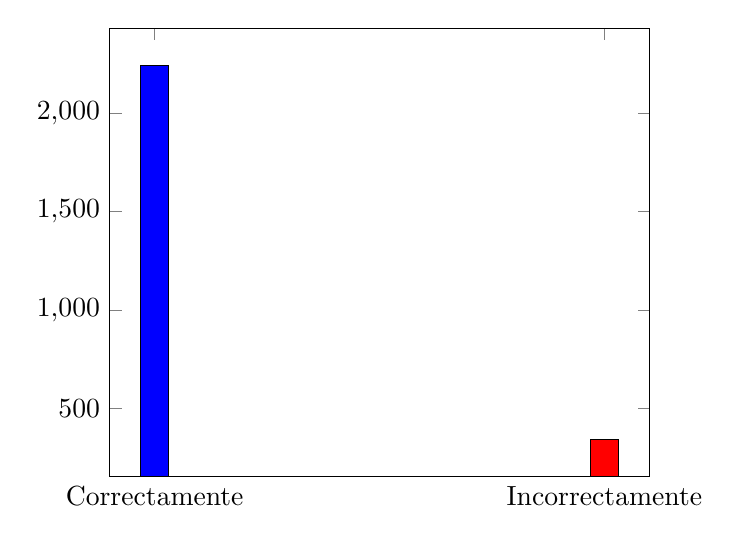
\begin{tikzpicture}
   
        \begin{axis}[
            symbolic x coords={Correctamente,Incorrectamente},
            xtick=data
          ]
          \addplot[ybar,fill=blue] coordinates {
                (Correctamente, 2241)
                (Incorrectamente,343)
            };
           \addplot[ybar,fill=red] coordinates {
              
                (Incorrectamente,343)
            };

        \end{axis}
    \end{tikzpicture}
     \caption{Gráfico de resultados del conjunto de datos Seismic bump}
     
\end{figure}
%%%%%%%%%%%%%%%%%%%%%%%%
% 3. Percentage Split  %
%%%%%%%%%%%%%%%%%%%%%%%%
\subsubsection{Percentage Split}
%%%%%%%%%%%%%%%%%%%%%%%%%%%%%%%
%Sección de Percentage Split  %
%%%%%%%%%%%%%%%%%%%%%%%%%%%%%%%
%%%%%%%%%%%%%%%%%%%%%%%%
% 4. Supplied test set %
%%%%%%%%%%%%%%%%%%%%%%%%
\subsubsection{Supplied test set}
%%%%%%%%%%%%%%%%%%%%%%%%%%%%%%%
%Sección de Supplied test set %
%%%%%%%%%%%%%%%%%%%%%%%%%%%%%%%
%%%%%%%%%%%%%%%%%%%%%%%%
% 5. Conclusiones %
%%%%%%%%%%%%%%%%%%%%%%%%
\subsubsection{Conclusiones}
%%%%%%%%%%%%%%%
%Conclusiones %
%%%%%%%%%%%%%%%
Es preciso decir que para el conjunto de datos Seismic-bump, fue efectiva la clasificación por medio del clasificador Naïve Bayes, debido a que el porcentaje de instancias clasificadas correctamente es mayor al número de instancias clasificadas incorrectamente.
%%%%%%%%%%%%%%%%%%%%%%%%
% Arboles de decisión  %
%%%%%%%%%%%%%%%%%%%%%%%%
\subsection{Arboles de decisión}
%%%%%%%%%%%%%%%%%%%%%%%%%%%%%%%
%Sección Arboles de decisión  %
%%%%%%%%%%%%%%%%%%%%%%%%%%%%%%%
%%%%%%%%%%%%%%%%%%%%%%%%
% 2. Cross-Validation  %
%%%%%%%%%%%%%%%%%%%%%%%%
\subsubsection{Cross-Validation}
%%%%%%%%%%%%%%%%%%%%%%%%%%%%%%%
%Sección de Cross-Validation  %
%%%%%%%%%%%%%%%%%%%%%%%%%%%%%%%
%%%%%%%%%%%%%%%%%%%%
% Redes neuronales %
%%%%%%%%%%%%%%%%%%%%
\subsection{Redes neuronales}
%%%%%%%%%%%%%%%%%%%%%%%%%%%%
%Sección Redes neuronales  %
%%%%%%%%%%%%%%%%%%%%%%%%%%%%
%%%%%%%%%%%%%%%%%%%%%%%%
% 2. Cross-Validation  %
%%%%%%%%%%%%%%%%%%%%%%%%
\subsubsection{Cross-Validation}
%%%%%%%%%%%%%%%%%%%%%%%%%%%%%%%
%Sección de Cross-Validation  %
%%%%%%%%%%%%%%%%%%%%%%%%%%%%%%%
%%%%%%%%%%%%%%%%
% K-Vecinos  %
%%%%%%%%%%%%%%%%
\subsection{K-Vecinos}
%%%%%%%%%%%%%%%%%%%%%%%
%Sección K-Vecinos  %
%%%%%%%%%%%%%%%%%%%%%%%
%%%%%%%%%%%%%%%%%%%%%%%%
% 2. Cross-Validation  %
%%%%%%%%%%%%%%%%%%%%%%%%
\subsubsection{Cross-Validation}
%%%%%%%%%%%%%%%%%%%%%%%%%%%%%%%
%Sección de Cross-Validation  %
%%%%%%%%%%%%%%%%%%%%%%%%%%%%%%%
%%%%%%%%%%%%%%%%%%%%%%%%%%%%%%%%%%%%
% Máquinas de vectores de soporte  %
%%%%%%%%%%%%%%%%%%%%%%%%%%%%%%%%%%%%
\subsection{Máquinas de vectores de soporte}
%%%%%%%%%%%%%%%%%%%%%%%
%Sección Máquinas de vectores de soporte  %
%%%%%%%%%%%%%%%%%%%%%%%
%%%%%%%%%%%%%%%%%%%%%%%%
% 2. Cross-Validation  %
%%%%%%%%%%%%%%%%%%%%%%%%
\subsubsection{Cross-Validation}
%%%%%%%%%%%%%%%%%%%%%%%%%%%%%%%
%Sección de Cross-Validation  %
%%%%%%%%%%%%%%%%%%%%%%%%%%%%%%%
%%%%%%%%%%%%%%%%%%%%%%%%%%%%%
%    7. Gama mágica telescopio   %
%%%%%%%%%%%%%%%%%%%%%%%%%%%%%
\section{Gama mágica telescopio}
%%%%%%%%%%%%%%%%%%%%%%%%%%%%%%%%%%%%%%
%Sección de Gama mágica telescopio    %
%%%%%%%%%%%%%%%%%%%%%%%%%%%%%%%%%%%%%%
Los datos son generados MC (ver más abajo) para simular el registro de partículas de alta energía gamma en un telescopio atmosférica gamma de Cherenkov con base en tierra utilizando la técnica de formación de imágenes. Telescopio gamma de Cherenkov observa rayos gamma de alta energía, tomando ventaja de la radiación emitida por las partículas cargadas producidas en el interior de las duchas electromagnéticas iniciadas por las gammas, y el desarrollo en la atmósfera. Esta radiación Cherenkov (de visible a longitudes de onda UV) se filtra a través de la atmósfera y se graba en el detector , lo que permite la reconstrucción de los parámetros de la ducha . La información disponible se compone de pulsos dejados por los fotones Cherenkov entrantes en los tubos fotomultiplicadores, dispuestos en un plano, la cámara. Dependiendo de la energía de la gamma primaria, un total de unos pocos cientos a unos 10.000 fotones Cherenkov conseguir recoge, en patrones (llamados la imagen ducha) , lo que permite discriminar estadísticamente las causadas por radiaciones gamma primarios (señal) de las imágenes de duchas hadrónicas inició por los rayos cósmicos en la atmósfera superior (fondo) .
Típicamente, la imagen de una ducha después de algún procesamiento previo es un racimo alargado. Su eje longitudinal está orientado hacia el centro de la cámara si el eje de la ducha es paralelo al eje óptico del telescopio, es decir, si el eje del telescopio se dirige hacia una fuente de punto. Un análisis de componentes principales se lleva a cabo en el plano de la cámara, lo que resulta en un eje de correlación y define una elipse. Si las deposiciones se distribuyeron como gaussiana bi variante, esto sería una elipse equidensity. Los parámetros característicos de esta elipse (a menudo llamadas parámetros Hilla) son algunos de los parámetros de imagen que pueden ser utilizados para la discriminación. Las deposiciones de energía son típicamente asimétrica a lo largo del eje mayor, y esta asimetría también puede ser utilizada en la discriminación. Hay, además, discriminar aún más características, como la medida de la agrupación en el plano de la imagen, o la suma total de las deposiciones.
%%%%%%%%%%%%%%%%%%%%%%%%%%%%%%%%%%%%%%%%%%%%%%%%%%%%%%%
% Tabla de Instancias y número de atributos %
%%%%%%%%%%%%%%%%%%%%%%%%%%%%%%%%%%%%%%%%%%%%%%%%%%%%%%%
\begin{table}
\caption{Número de Instancias y Atributos de Gama mágica telescopio} % titulo de la tabla
\centering % es usado para centrar la tabla
\begin{tabular}{c c}
% columnas centradas (2 columnas)
\hline\hline %inserts double horizontal lines
Instancias & Atributos \\ [0.5ex]
% inserta tablas
%heading
\hline % Inserta una linea horizontal
19020 & 11 \\ [1ex] % [1ex] Agrega un espacio vertical
\hline %Inserta una linea
\end{tabular}
\label{table:gamatelescopioia} % Es usado para referise a esta tabla en el texto
\end{table}
%%%%%%%%%%%%%%%%%%%%
% Finaliza la tabla%
%%%%%%%%%%%%%%%%%%%%

%%%%%%%%%%%%%%%%%%%%%%%%%%%%%%%%%%%%%%%%%%%%%%%%%%%%%%%
% Atributos de Gama mágica telescopio  	              %
%%%%%%%%%%%%%%%%%%%%%%%%%%%%%%%%%%%%%%%%%%%%%%%%%%%%%%%
\begin{table}
\caption{Atributos de Gama mágica telescopio} % titulo de la tabla
\centering % es usado para centrar la tabla
\begin{tabular}{c c c}
% columnas centradas (3 columnas)
\hline\hline %inserts double horizontal lines
Atributo & Tipo & Dominio \\ [0.5ex]
% inserta tablas
%heading
\hline % Inserta una linea horizontal
Eje ancho	& Real& 	18-50\\ [1ex] % [1ex] Agrega un espacio vertical
Eje menor	& Real& 	1-4\\ [1ex] % [1ex] Agrega un espacio vertical
Log todos pixeles	& Binario & 	1,0\\ [1ex] % [1ex] Agrega un espacio vertical
Suma 2 pixeles	& Real& 	0.2323-0.24313\\ [1ex] % [1ex] Agrega un espacio vertical
Pixel mas alto	& Real& 	1,2,3,4\\ [1ex] % [1ex] Agrega un espacio vertical
Distancia pixel alto	& Real.& 	0.365, 0.600, 0.666, etc.\\ [1ex] % [1ex] Agrega un espacio vertical
longitud mayor	& Real& 	1.2, 0.4678, …\\ [1ex] % [1ex] Agrega un espacio vertical
longitud menor	& Real& 	0.4755, 0.45, 0.33, …\\ [1ex] % [1ex] Agrega un espacio vertical
Angulo	& Real& 	0.4755, 0.4005, 0.3233, …\\ [1ex] % [1ex] Agrega un espacio vertical
Distancia	& Real& 	0.365, 0.444, 0.3200, …\\ [1ex] % [1ex] Agrega un espacio vertical
clases	& Real & 	4,5…,10, 19,… etc.\\ [1ex] % [1ex] Agrega un espacio vertical
\hline %Inserta una linea
\end{tabular}
\label{table:gamatelescopioa} % Es usado para referise a esta tabla en el texto
\end{table}
%%%%%%%%%%%%%%%%%%%%
% Finaliza la tabla%
%%%%%%%%%%%%%%%%%%%%
%%%%%%%%%%%%%%%%
% Naïve Bayes  %
%%%%%%%%%%%%%%%%
\subsection{Naïve Bayes}
%%%%%%%%%%%%%%%%%%%%%%%
%Sección Naïve Bayes  %
%%%%%%%%%%%%%%%%%%%%%%%
%%%%%%%%%%%%%%%%%%%%%%%%
% 1. Use training set  %
%%%%%%%%%%%%%%%%%%%%%%%%
\subsubsection{Use training set}
%%%%%%%%%%%%%%%%%%%%%%%%%%%%%%%
%Sección de Use training set  %
%%%%%%%%%%%%%%%%%%%%%%%%%%%%%%%
%%%%%%%%%%%%%%%%%%%%%%%%
% 2. Cross-Validation  %
%%%%%%%%%%%%%%%%%%%%%%%%
\subsubsection{Cross-Validation}
%%%%%%%%%%%%%%%%%%%%%%%%%%%%%%%
%Sección de Cross-Validation  %
%%%%%%%%%%%%%%%%%%%%%%%%%%%%%%%
\begin{figure}[h!]
 \centering
    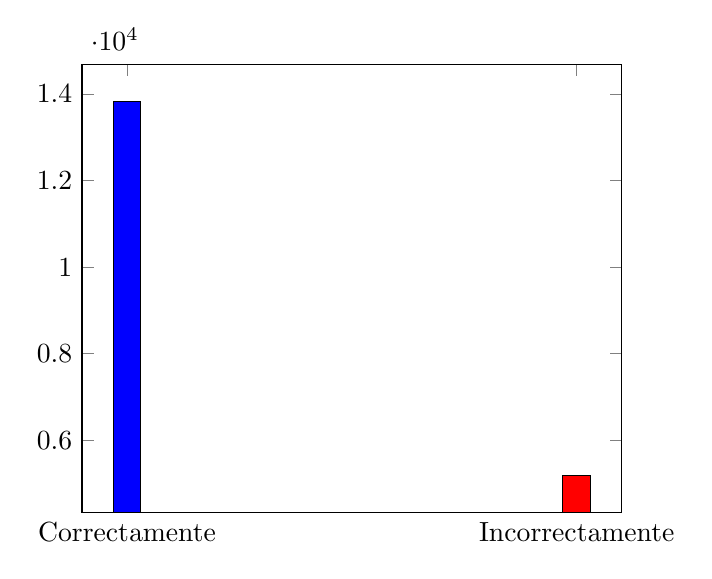
\begin{tikzpicture}
   
        \begin{axis}[
            symbolic x coords={Correctamente,Incorrectamente},
            xtick=data
          ]
          \addplot[ybar,fill=blue] coordinates {
                (Correctamente, 13825)
                (Incorrectamente,5195)
            };
           \addplot[ybar,fill=red] coordinates {
              
                (Incorrectamente,5195)
            };

        \end{axis}
    \end{tikzpicture}
     \caption{Gráfico de resultados del conjunto de datos Gama mágica telescopio}
     
\end{figure}
%%%%%%%%%%%%%%%%%%%%%%%%
% 3. Percentage Split  %
%%%%%%%%%%%%%%%%%%%%%%%%
\subsubsection{Percentage Split}
%%%%%%%%%%%%%%%%%%%%%%%%%%%%%%%
%Sección de Percentage Split  %
%%%%%%%%%%%%%%%%%%%%%%%%%%%%%%%
%%%%%%%%%%%%%%%%%%%%%%%%
% 4. Supplied test set %
%%%%%%%%%%%%%%%%%%%%%%%%
\subsubsection{Supplied test set}
%%%%%%%%%%%%%%%%%%%%%%%%%%%%%%%
%Sección de Supplied test set %
%%%%%%%%%%%%%%%%%%%%%%%%%%%%%%%
%%%%%%%%%%%%%%%%%%%%%%%%
% 5. Conclusiones %
%%%%%%%%%%%%%%%%%%%%%%%%
\subsubsection{Conclusiones}
%%%%%%%%%%%%%%%
%Conclusiones %
%%%%%%%%%%%%%%%
Es preciso decir que para el conjunto de datos Gama mágica telescopio, fue efectiva la clasificación por medio del clasificador Naïve Bayes, debido a que el porcentaje de instancias clasificadas correctamente es mayor al número de instancias clasificadas incorrectamente.
%%%%%%%%%%%%%%%%%%%%%%%%
% Arboles de decisión  %
%%%%%%%%%%%%%%%%%%%%%%%%
\subsection{Arboles de decisión}
%%%%%%%%%%%%%%%%%%%%%%%%%%%%%%%
%Sección Arboles de decisión  %
%%%%%%%%%%%%%%%%%%%%%%%%%%%%%%%
%%%%%%%%%%%%%%%%%%%%%%%%
% 2. Cross-Validation  %
%%%%%%%%%%%%%%%%%%%%%%%%
\subsubsection{Cross-Validation}
%%%%%%%%%%%%%%%%%%%%%%%%%%%%%%%
%Sección de Cross-Validation  %
%%%%%%%%%%%%%%%%%%%%%%%%%%%%%%%
%%%%%%%%%%%%%%%%%%%%
% Redes neuronales %
%%%%%%%%%%%%%%%%%%%%
\subsection{Redes neuronales}
%%%%%%%%%%%%%%%%%%%%%%%%%%%%
%Sección Redes neuronales  %
%%%%%%%%%%%%%%%%%%%%%%%%%%%%
%%%%%%%%%%%%%%%%%%%%%%%%
% 2. Cross-Validation  %
%%%%%%%%%%%%%%%%%%%%%%%%
\subsubsection{Cross-Validation}
%%%%%%%%%%%%%%%%%%%%%%%%%%%%%%%
%Sección de Cross-Validation  %
%%%%%%%%%%%%%%%%%%%%%%%%%%%%%%%
%%%%%%%%%%%%%%%%
% K-Vecinos  %
%%%%%%%%%%%%%%%%
\subsection{K-Vecinos}
%%%%%%%%%%%%%%%%%%%%%%%
%Sección K-Vecinos  %
%%%%%%%%%%%%%%%%%%%%%%%
%%%%%%%%%%%%%%%%%%%%%%%%
% 2. Cross-Validation  %
%%%%%%%%%%%%%%%%%%%%%%%%
\subsubsection{Cross-Validation}
%%%%%%%%%%%%%%%%%%%%%%%%%%%%%%%
%Sección de Cross-Validation  %
%%%%%%%%%%%%%%%%%%%%%%%%%%%%%%%
%%%%%%%%%%%%%%%%%%%%%%%%%%%%%%%%%%%%
% Máquinas de vectores de soporte  %
%%%%%%%%%%%%%%%%%%%%%%%%%%%%%%%%%%%%
\subsection{Máquinas de vectores de soporte}
%%%%%%%%%%%%%%%%%%%%%%%
%Sección Máquinas de vectores de soporte  %
%%%%%%%%%%%%%%%%%%%%%%%
%%%%%%%%%%%%%%%%%%%%%%%%
% 2. Cross-Validation  %
%%%%%%%%%%%%%%%%%%%%%%%%
\subsubsection{Cross-Validation}
%%%%%%%%%%%%%%%%%%%%%%%%%%%%%%%
%Sección de Cross-Validation  %
%%%%%%%%%%%%%%%%%%%%%%%%%%%%%%%
%%%%%%%%%%%%%%%%%%%%%%%%%%%%%
%    8. Método Anticonceptivo   %
%%%%%%%%%%%%%%%%%%%%%%%%%%%%%
\section{Método Anticonceptivo}
%%%%%%%%%%%%%%%%%%%%%%%%%%%%%%%%%%%%%%
%Sección de Método Anticonceptivo    %
%%%%%%%%%%%%%%%%%%%%%%%%%%%%%%%%%%%%%%
Este conjunto de datos es un subconjunto de la encuesta  de Las muestras son mujeres casadas que eran o no embarazada o no saben si se encontraban en el momento de la entrevista. El problema es predecir la elección actual método anticonceptivo (sin uso, métodos de largo plazo, o los métodos de corto plazo) de una mujer sobre la base de sus características demográficas y socio-económicas.
%%%%%%%%%%%%%%%%%%%%%%%%%%%%%%%%%%%%%%%%%%%%%%%%%%%%%%%
% Tabla de Instancias y número de atributos %
%%%%%%%%%%%%%%%%%%%%%%%%%%%%%%%%%%%%%%%%%%%%%%%%%%%%%%%
\begin{table}
\caption{Número de Instancias y Atributos de Método anticonceptivo} % titulo de la tabla
\centering % es usado para centrar la tabla
\begin{tabular}{c c}
% columnas centradas (2 columnas)
\hline\hline %inserts double horizontal lines
Instancias & Atributos \\ [0.5ex]
% inserta tablas
%heading
\hline % Inserta una linea horizontal
1473 & 10 \\ [1ex] % [1ex] Agrega un espacio vertical
\hline %Inserta una linea
\end{tabular}
\label{table:metodoanticonceptivoia} % Es usado para referise a esta tabla en el texto
\end{table}
%%%%%%%%%%%%%%%%%%%%
% Finaliza la tabla%
%%%%%%%%%%%%%%%%%%%%
%%%%%%%%%%%%%%%%%%%%%%%%%%%%%%%%%%%%%%%%%%%%%%%%%%%%%%%
% Atributos de Método anticonceptivo 	              %
%%%%%%%%%%%%%%%%%%%%%%%%%%%%%%%%%%%%%%%%%%%%%%%%%%%%%%%
\begin{table}
\caption{Atributos de Método anticonceptivo } % titulo de la tabla
\centering % es usado para centrar la tabla
\begin{tabular}{c c c}
% columnas centradas (3 columnas)
\hline\hline %inserts double horizontal lines
Atributo & Tipo & Dominio \\ [0.5ex]
% inserta tablas
%heading
\hline % Inserta una linea horizontal
Edad de la esposa	& Numérico& 	18-50\\ [1ex] % [1ex] Agrega un espacio vertical
La educación de la esposa	& Real& 	1-4\\ [1ex] % [1ex] Agrega un espacio vertical
La educación del esposo	& Real& 	1-4\\ [1ex] % [1ex] Agrega un espacio vertical
Número de hijos nacidos vivos & Numérico &	1-10\\ [1ex] % [1ex] Agrega un espacio vertical
La religión de la esposa	& Real & 	0,1\\ [1ex] % [1ex] Agrega un espacio vertical
¿Esposa Ahora está trabajando?	& Binario & 	0,1\\ [1ex] % [1ex] Agrega un espacio vertical
Ocupación del esposo	& Real& 	1-4\\ [1ex] % [1ex] Agrega un espacio vertical
Esperanza de vida	& Real& 	1-4\\ [1ex] % [1ex] Agrega un espacio vertical
Exposición a los medios	& Binario &   1,0\\ [1ex] % [1ex] Agrega un espacio vertical
Clase	& Real &  1,2,3\\ [1ex] % [1ex] Agrega un espacio vertical
\hline %Inserta una linea
\end{tabular}
\label{table:metodoanticonceptivoa} % Es usado para referise a esta tabla en el texto
\end{table}
%%%%%%%%%%%%%%%%%%%%
% Finaliza la tabla%
%%%%%%%%%%%%%%%%%%%%
%%%%%%%%%%%%%%%%
% Naïve Bayes  %
%%%%%%%%%%%%%%%%
\subsection{Naïve Bayes}
%%%%%%%%%%%%%%%%%%%%%%%
%Sección Naïve Bayes  %
%%%%%%%%%%%%%%%%%%%%%%%
%%%%%%%%%%%%%%%%%%%%%%%%
% 1. Use training set  %
%%%%%%%%%%%%%%%%%%%%%%%%
\subsubsection{Use training set}
%%%%%%%%%%%%%%%%%%%%%%%%%%%%%%%
%Sección de Use training set  %
%%%%%%%%%%%%%%%%%%%%%%%%%%%%%%%
%%%%%%%%%%%%%%%%%%%%%%%%
% 2. Cross-Validation  %
%%%%%%%%%%%%%%%%%%%%%%%%
\subsubsection{Cross-Validation}
%%%%%%%%%%%%%%%%%%%%%%%%%%%%%%%
%Sección de Cross-Validation  %
%%%%%%%%%%%%%%%%%%%%%%%%%%%%%%%
\begin{figure}[h!]
 \centering
    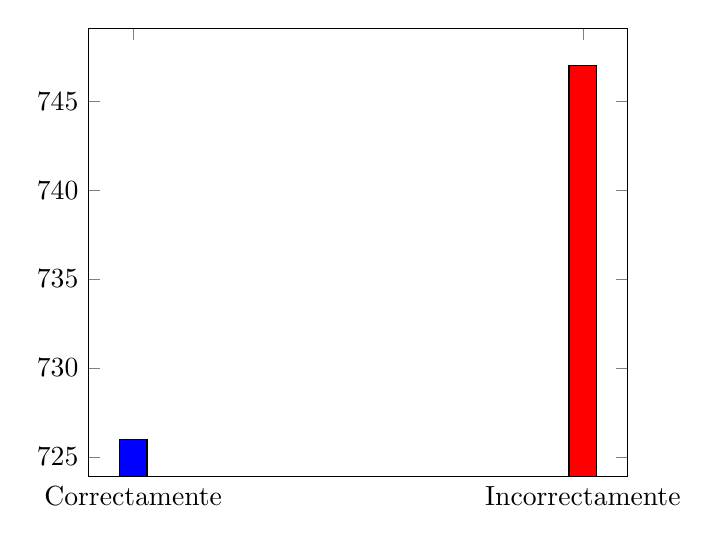
\begin{tikzpicture}
   
        \begin{axis}[
            symbolic x coords={Correctamente,Incorrectamente},
            xtick=data
          ]
          \addplot[ybar,fill=blue] coordinates {
                (Correctamente, 726)
                (Incorrectamente,747)
            };
           \addplot[ybar,fill=red] coordinates {
              
                (Incorrectamente,747)
            };

        \end{axis}
    \end{tikzpicture}
     \caption{Gráfico de resultados del conjunto de datos Método anticonceptivo}
     
\end{figure}
%%%%%%%%%%%%%%%%%%%%%%%%
% 3. Percentage Split  %
%%%%%%%%%%%%%%%%%%%%%%%%
\subsubsection{Percentage Split}
%%%%%%%%%%%%%%%%%%%%%%%%%%%%%%%
%Sección de Percentage Split  %
%%%%%%%%%%%%%%%%%%%%%%%%%%%%%%%
%%%%%%%%%%%%%%%%%%%%%%%%
% 4. Supplied test set %
%%%%%%%%%%%%%%%%%%%%%%%%
\subsubsection{Supplied test set}
%%%%%%%%%%%%%%%%%%%%%%%%%%%%%%%
%Sección de Supplied test set %
%%%%%%%%%%%%%%%%%%%%%%%%%%%%%%%
\subsubsection{Conclusiones}
%%%%%%%%%%%%%%%
%Conclusiones %
%%%%%%%%%%%%%%%
Es preciso decir que para el conjunto de datos Método anticonceptivo, no fue efectiva la clasificación por medio del clasificador Naïve Bayes, debido a que el porcentaje de instancias clasificadas correctamente es similar al número de instancias clasificadas incorrectamente.
%%%%%%%%%%%%%%%%%%%%%%%%
% Arboles de decisión  %
%%%%%%%%%%%%%%%%%%%%%%%%
\subsection{Arboles de decisión}
%%%%%%%%%%%%%%%%%%%%%%%%%%%%%%%
%Sección Arboles de decisión  %
%%%%%%%%%%%%%%%%%%%%%%%%%%%%%%%
%%%%%%%%%%%%%%%%%%%%%%%%
% 2. Cross-Validation  %
%%%%%%%%%%%%%%%%%%%%%%%%
\subsubsection{Cross-Validation}
%%%%%%%%%%%%%%%%%%%%%%%%%%%%%%%
%Sección de Cross-Validation  %
%%%%%%%%%%%%%%%%%%%%%%%%%%%%%%%
%%%%%%%%%%%%%%%%%%%%
% Redes neuronales %
%%%%%%%%%%%%%%%%%%%%
\subsection{Redes neuronales}
%%%%%%%%%%%%%%%%%%%%%%%%%%%%
%Sección Redes neuronales  %
%%%%%%%%%%%%%%%%%%%%%%%%%%%%
%%%%%%%%%%%%%%%%%%%%%%%%
% 2. Cross-Validation  %
%%%%%%%%%%%%%%%%%%%%%%%%
\subsubsection{Cross-Validation}
%%%%%%%%%%%%%%%%%%%%%%%%%%%%%%%
%Sección de Cross-Validation  %
%%%%%%%%%%%%%%%%%%%%%%%%%%%%%%%
%%%%%%%%%%%%%%%%
% K-Vecinos  %
%%%%%%%%%%%%%%%%
\subsection{K-Vecinos}
%%%%%%%%%%%%%%%%%%%%%%%
%Sección K-Vecinos  %
%%%%%%%%%%%%%%%%%%%%%%%
%%%%%%%%%%%%%%%%%%%%%%%%
% 2. Cross-Validation  %
%%%%%%%%%%%%%%%%%%%%%%%%
\subsubsection{Cross-Validation}
%%%%%%%%%%%%%%%%%%%%%%%%%%%%%%%
%Sección de Cross-Validation  %
%%%%%%%%%%%%%%%%%%%%%%%%%%%%%%%
%%%%%%%%%%%%%%%%%%%%%%%%%%%%%%%%%%%%
% Máquinas de vectores de soporte  %
%%%%%%%%%%%%%%%%%%%%%%%%%%%%%%%%%%%%
\subsection{Máquinas de vectores de soporte}
%%%%%%%%%%%%%%%%%%%%%%%
%Sección Máquinas de vectores de soporte  %
%%%%%%%%%%%%%%%%%%%%%%%
%%%%%%%%%%%%%%%%%%%%%%%%
% 2. Cross-Validation  %
%%%%%%%%%%%%%%%%%%%%%%%%
\subsubsection{Cross-Validation}
%%%%%%%%%%%%%%%%%%%%%%%%%%%%%%%
%Sección de Cross-Validation  %
%%%%%%%%%%%%%%%%%%%%%%%%%%%%%%%
%%%%%%%%%%%%%%%%%%%%%%%%%%%%%
%    9. Letter Recognition   %
%%%%%%%%%%%%%%%%%%%%%%%%%%%%%
\section{Letter Recognition}
%%%%%%%%%%%%%%%%%%%%%%%%%%%%%%%%%%%%%%
%Sección de Letter Recognition    %
%%%%%%%%%%%%%%%%%%%%%%%%%%%%%%%%%%%%%%
El objetivo de esta base de datos es identificar cada número grande de un rectángulo en blanco y negro como una de las 26 letras capitales en el alfabeto inglés. Los caracteres fueron basados en 20 diferentes fuentes y cada letra dentro de éstas 20 fuentes fue aleatoriamente alterada, distorsionada, para producir un archivo de 20,000 estímulos únicos. Cada estímulo fue convertido en 16 atributos numéricos, los cuales fueron escalados para ajustarlos dentro de un rango de valores enteros (de 0 a 15).
%%%%%%%%%%%%%%%%%%%%%%%%%%%%%%%%%%%%%%%%%%%%%%%%%%%%%%%
% Tabla de Instancias y número de atributos %
%%%%%%%%%%%%%%%%%%%%%%%%%%%%%%%%%%%%%%%%%%%%%%%%%%%%%%%
\begin{table}
\caption{Número de Instancias y Atributos de Letter Recognition} % titulo de la tabla
\centering % es usado para centrar la tabla
\begin{tabular}{c c}
% columnas centradas (2 columnas)
\hline\hline %inserts double horizontal lines
Instancias & Atributos \\ [0.5ex]
% inserta tablas
%heading
\hline % Inserta una linea horizontal
20000 & 17 \\ [1ex] % [1ex] Agrega un espacio vertical
\hline %Inserta una linea
\end{tabular}
\label{table:letterrecognitionia} % Es usado para referise a esta tabla en el texto
\end{table}
%%%%%%%%%%%%%%%%%%%%
% Finaliza la tabla%
%%%%%%%%%%%%%%%%%%%%
%%%%%%%%%%%%%%%%%%%%%%%%%%%%%%%%%%%%%%%%%%%%%%%%%%%%%%%
% Atributos de Letter Recognition    	              %
%%%%%%%%%%%%%%%%%%%%%%%%%%%%%%%%%%%%%%%%%%%%%%%%%%%%%%%
\begin{table}
\caption{Atributos de Letter Recognition} % titulo de la tabla
\centering % es usado para centrar la tabla
\begin{tabular}{c c c}
% columnas centradas (3 columnas)
\hline\hline %inserts double horizontal lines
Atributo & Tipo & Dominio \\ [0.5ex]
% inserta tablas
%heading
\hline % Inserta una linea horizontal
Clase	& Categórico & 	{A,B,C,D,E,…,X,Y,Z}\\ [1ex] % [1ex] Agrega un espacio vertical
Poscajax hor	& Numérico& 	9,10,7,3,…\\ [1ex] % [1ex] Agrega un espacio vertical
Poscajay ver	& Numérico& 	9,10,7,3,…\\ [1ex] % [1ex] Agrega un espacio vertical
Ancho caja	& Numérico& 	9,10,7,3,…\\ [1ex] % [1ex] Agrega un espacio vertical
Altura caja	& Numérico& 	9,10,7,3,…\\ [1ex] % [1ex] Agrega un espacio vertical
totalpix	& Numérico& 	9,10,7,3,…\\ [1ex] % [1ex] Agrega un espacio vertical
Barrax	& Numérico& 	9,10,7,3,…\\ [1ex] % [1ex] Agrega un espacio vertical
Barray	& Numérico& 	9,10,7,3,…\\ [1ex] % [1ex] Agrega un espacio vertical
Barrax2	& Numérico& 	9,10,7,3,…\\ [1ex] % [1ex] Agrega un espacio vertical
Barray2	& Numérico& 	9,10,7,3,…\\ [1ex] % [1ex] Agrega un espacio vertical
barraxy	& Numérico& 	9,10,7,3,…\\ [1ex] % [1ex] Agrega un espacio vertical
x2ybr	& Numérico& 	9,10,7,3,…\\ [1ex] % [1ex] Agrega un espacio vertical
xy2br	& Numérico& 	9,10,7,3,…\\ [1ex] % [1ex] Agrega un espacio vertical
x esquina	& Numérico& 	9,10,7,3,…\\ [1ex] % [1ex] Agrega un espacio vertical
Xegvy	& Numérico& 	9,10,7,3,…\\ [1ex] % [1ex] Agrega un espacio vertical
y esquina	& Numérico& 	9,10,7,3,…\\ [1ex] % [1ex] Agrega un espacio vertical
yegvx	& Numérico	& 9,10,7,3,…\\ [1ex] % [1ex] Agrega un espacio vertical
\hline %Inserta una linea
\end{tabular}
\label{table:letterrecognitiona} % Es usado para referise a esta tabla en el texto
\end{table}
%%%%%%%%%%%%%%%%%%%%
% Finaliza la tabla%
%%%%%%%%%%%%%%%%%%%%
%%%%%%%%%%%%%%%%
% Naïve Bayes  %
%%%%%%%%%%%%%%%%
\subsection{Naïve Bayes}
%%%%%%%%%%%%%%%%%%%%%%%
%Sección Naïve Bayes  %
%%%%%%%%%%%%%%%%%%%%%%%
%%%%%%%%%%%%%%%%%%%%%%%%
% 1. Use training set  %
%%%%%%%%%%%%%%%%%%%%%%%%
\subsubsection{Use training set}
%%%%%%%%%%%%%%%%%%%%%%%%%%%%%%%
%Sección de Use training set  %
%%%%%%%%%%%%%%%%%%%%%%%%%%%%%%%
%%%%%%%%%%%%%%%%%%%%%%%%
% 2. Cross-Validation  %
%%%%%%%%%%%%%%%%%%%%%%%%
\subsubsection{Cross-Validation}
%%%%%%%%%%%%%%%%%%%%%%%%%%%%%%%
%Sección de Cross-Validation  %
%%%%%%%%%%%%%%%%%%%%%%%%%%%%%%%
\begin{figure}[h!]
 \centering
    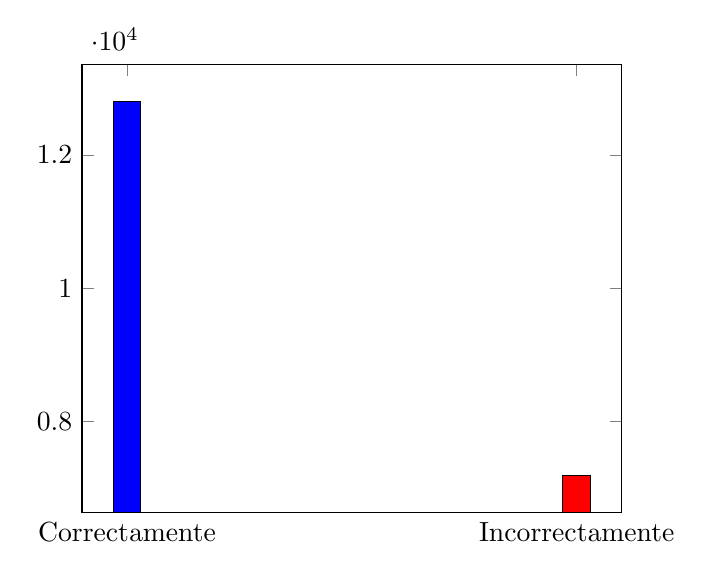
\begin{tikzpicture}
   
        \begin{axis}[
            symbolic x coords={Correctamente,Incorrectamente},
            xtick=data
          ]
          \addplot[ybar,fill=blue] coordinates {
                (Correctamente, 12802)
                (Incorrectamente,7198)
            };
           \addplot[ybar,fill=red] coordinates {
              
                (Incorrectamente,7198)
            };

        \end{axis}
    \end{tikzpicture}
     \caption{Gráfico de resultados del conjunto de datos Letter Recognition}
     
\end{figure}
%%%%%%%%%%%%%%%%%%%%%%%%
% 3. Percentage Split  %
%%%%%%%%%%%%%%%%%%%%%%%%
\subsubsection{Percentage Split}
%%%%%%%%%%%%%%%%%%%%%%%%%%%%%%%
%Sección de Percentage Split  %
%%%%%%%%%%%%%%%%%%%%%%%%%%%%%%%
%%%%%%%%%%%%%%%%%%%%%%%%
% 4. Supplied test set %
%%%%%%%%%%%%%%%%%%%%%%%%
\subsubsection{Supplied test set}
%%%%%%%%%%%%%%%%%%%%%%%%%%%%%%%
%Sección de Supplied test set %
%%%%%%%%%%%%%%%%%%%%%%%%%%%%%%%
%%%%%%%%%%%%%%%%%%%%%%%%
% 5. Conclusiones %
%%%%%%%%%%%%%%%%%%%%%%%%
\subsubsection{Conclusiones}
%%%%%%%%%%%%%%%
%Conclusiones %
%%%%%%%%%%%%%%%
Es preciso decir que para el conjunto de datos Letter Recognition, fue efectiva la clasificación por medio del clasificador Naïve Bayes, debido a que el porcentaje de instancias clasificadas correctamente es mayor al número de instancias clasificadas incorrectamente.
%%%%%%%%%%%%%%%%%%%%%%%%
% Arboles de decisión  %
%%%%%%%%%%%%%%%%%%%%%%%%
\subsection{Arboles de decisión}
%%%%%%%%%%%%%%%%%%%%%%%%%%%%%%%
%Sección Arboles de decisión  %
%%%%%%%%%%%%%%%%%%%%%%%%%%%%%%%
%%%%%%%%%%%%%%%%%%%%%%%%
% 2. Cross-Validation  %
%%%%%%%%%%%%%%%%%%%%%%%%
\subsubsection{Cross-Validation}
%%%%%%%%%%%%%%%%%%%%%%%%%%%%%%%
%Sección de Cross-Validation  %
%%%%%%%%%%%%%%%%%%%%%%%%%%%%%%%
%%%%%%%%%%%%%%%%%%%%
% Redes neuronales %
%%%%%%%%%%%%%%%%%%%%
\subsection{Redes neuronales}
%%%%%%%%%%%%%%%%%%%%%%%%%%%%
%Sección Redes neuronales  %
%%%%%%%%%%%%%%%%%%%%%%%%%%%%
%%%%%%%%%%%%%%%%%%%%%%%%
% 2. Cross-Validation  %
%%%%%%%%%%%%%%%%%%%%%%%%
\subsubsection{Cross-Validation}
%%%%%%%%%%%%%%%%%%%%%%%%%%%%%%%
%Sección de Cross-Validation  %
%%%%%%%%%%%%%%%%%%%%%%%%%%%%%%%
%%%%%%%%%%%%%%%%
% K-Vecinos  %
%%%%%%%%%%%%%%%%
\subsection{K-Vecinos}
%%%%%%%%%%%%%%%%%%%%%%%
%Sección K-Vecinos  %
%%%%%%%%%%%%%%%%%%%%%%%
%%%%%%%%%%%%%%%%%%%%%%%%
% 2. Cross-Validation  %
%%%%%%%%%%%%%%%%%%%%%%%%
\subsubsection{Cross-Validation}
%%%%%%%%%%%%%%%%%%%%%%%%%%%%%%%
%Sección de Cross-Validation  %
%%%%%%%%%%%%%%%%%%%%%%%%%%%%%%%
%%%%%%%%%%%%%%%%%%%%%%%%%%%%%%%%%%%%
% Máquinas de vectores de soporte  %
%%%%%%%%%%%%%%%%%%%%%%%%%%%%%%%%%%%%
\subsection{Máquinas de vectores de soporte}
%%%%%%%%%%%%%%%%%%%%%%%
%Sección Máquinas de vectores de soporte  %
%%%%%%%%%%%%%%%%%%%%%%%
%%%%%%%%%%%%%%%%%%%%%%%%
% 2. Cross-Validation  %
%%%%%%%%%%%%%%%%%%%%%%%%
\subsubsection{Cross-Validation}
%%%%%%%%%%%%%%%%%%%%%%%%%%%%%%%
%Sección de Cross-Validation  %
%%%%%%%%%%%%%%%%%%%%%%%%%%%%%%%
%%%%%%%%%%%%%%%%%%%%%%%%%%%%%
%    10. Banknote   %
%%%%%%%%%%%%%%%%%%%%%%%%%%%%%
\section{Banknote}
%%%%%%%%%%%%%%%%%%%%%%%%%%%%%%%%%%%%%%
%Sección de Banknote    %
%%%%%%%%%%%%%%%%%%%%%%%%%%%%%%%%%%%%%%
Los datos fueron extraídos de imágenes que fueron tomadas de los especímenes genuinos y falsificados y como de billetes de banco. Para la digitalización, una cámara fotográfica industrial usualmente destinada para inspección estampada fue usada. Las imágenes finales tienen a 400x 400 pixeles. Debido al lente del objeto y distancia para las fotos del objeto de escalas de grises investigadas con una decisión de aproximadamente 660 puntos por pulgada fue ganado. La herramienta de la ola pequeña Transform se usara para extractar características de imágenes.
%%%%%%%%%%%%%%%%%%%%%%%%%%%%%%%%%%%%%%%%%%%%%%%%%%%%%%%
% Tabla de Instancias y número de atributos %
%%%%%%%%%%%%%%%%%%%%%%%%%%%%%%%%%%%%%%%%%%%%%%%%%%%%%%%
\begin{table}
\caption{Número de Instancias y Atributos de Banknote} % titulo de la tabla
\centering % es usado para centrar la tabla
\begin{tabular}{c c}
% columnas centradas (2 columnas)
\hline\hline %inserts double horizontal lines
Instancias & Atributos \\ [0.5ex]
% inserta tablas
%heading
\hline % Inserta una linea horizontal
1372 & 5 \\ [1ex] % [1ex] Agrega un espacio vertical
\hline %Inserta una linea
\end{tabular}
\label{table:banknoteia} % Es usado para referise a esta tabla en el texto
\end{table}
%%%%%%%%%%%%%%%%%%%%
% Finaliza la tabla%
%%%%%%%%%%%%%%%%%%%%
%%%%%%%%%%%%%%%%%%%%%%%%%%%%%%%%%%%%%%%%%%%%%%%%%%%%%%%
% Atributos de Banknote              	              %
%%%%%%%%%%%%%%%%%%%%%%%%%%%%%%%%%%%%%%%%%%%%%%%%%%%%%%%
\begin{table}
\caption{Atributos de Banknote} % titulo de la tabla
\centering % es usado para centrar la tabla
\begin{tabular}{c c c}
% columnas centradas (3 columnas)
\hline\hline %inserts double horizontal lines
Atributo & Tipo & Dominio \\ [0.5ex]
% inserta tablas
%heading
\hline % Inserta una linea horizontal
varianza imagen	& Real & -8,..6\\ [1ex] % [1ex] Agrega un espacio vertical
asimetria imagen	& Real&  -14,..13	\\ [1ex] % [1ex] Agrega un espacio vertical
curtosis imagen	& Real & -6,..18\\ [1ex] % [1ex] Agrega un espacio vertical
entropia	& Real & -9,..3\\ [1ex] % [1ex] Agrega un espacio vertical
clase	& Real	& 0,1\\ [1ex] % [1ex] Agrega un espacio vertical
\hline %Inserta una linea
\end{tabular}
\label{table:banknotea} % Es usado para referise a esta tabla en el texto
\end{table}
%%%%%%%%%%%%%%%%%%%%
% Finaliza la tabla%
%%%%%%%%%%%%%%%%%%%%
%%%%%%%%%%%%%%%%
% Naïve Bayes  %
%%%%%%%%%%%%%%%%
\subsection{Naïve Bayes}
%%%%%%%%%%%%%%%%%%%%%%%
%Sección Naïve Bayes  %
%%%%%%%%%%%%%%%%%%%%%%%
%%%%%%%%%%%%%%%%%%%%%%%%
% 1. Use training set  %
%%%%%%%%%%%%%%%%%%%%%%%%
\subsubsection{Use training set}
%%%%%%%%%%%%%%%%%%%%%%%%%%%%%%%
%Sección de Use training set  %
%%%%%%%%%%%%%%%%%%%%%%%%%%%%%%%
%%%%%%%%%%%%%%%%%%%%%%%%
% 2. Cross-Validation  %
%%%%%%%%%%%%%%%%%%%%%%%%
\subsubsection{Cross-Validation}
%%%%%%%%%%%%%%%%%%%%%%%%%%%%%%%
%Sección de Cross-Validation  %
%%%%%%%%%%%%%%%%%%%%%%%%%%%%%%%
\begin{figure}[h!]
 \centering
    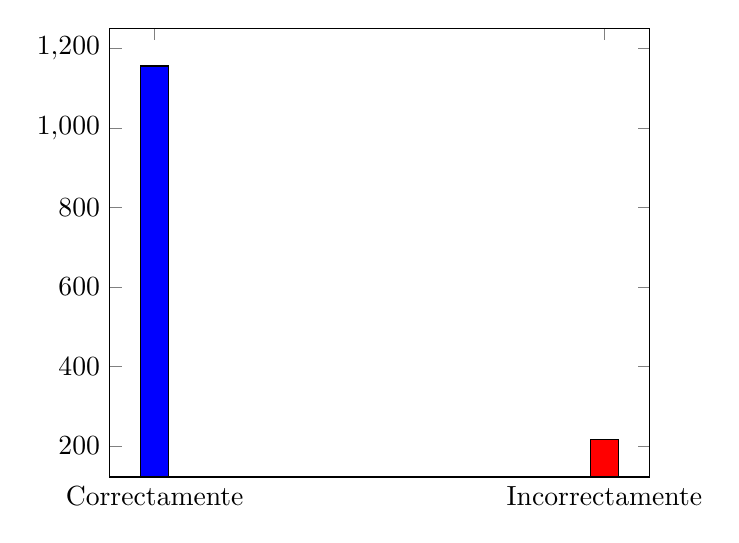
\begin{tikzpicture}
   
        \begin{axis}[
            symbolic x coords={Correctamente,Incorrectamente},
            xtick=data
          ]
          \addplot[ybar,fill=blue] coordinates {
                (Correctamente, 1156)
                (Incorrectamente,216)
            };
           \addplot[ybar,fill=red] coordinates {
              
                (Incorrectamente,216)
            };

        \end{axis}
    \end{tikzpicture}
     \caption{Gráfico de resultados del conjunto de datos Banknote}
     
\end{figure}
%%%%%%%%%%%%%%%%%%%%%%%%
% 3. Percentage Split  %
%%%%%%%%%%%%%%%%%%%%%%%%
\subsubsection{Percentage Split}
%%%%%%%%%%%%%%%%%%%%%%%%%%%%%%%
%Sección de Percentage Split  %
%%%%%%%%%%%%%%%%%%%%%%%%%%%%%%%
%%%%%%%%%%%%%%%%%%%%%%%%
% 4. Supplied test set %
%%%%%%%%%%%%%%%%%%%%%%%%
\subsubsection{Supplied test set}
%%%%%%%%%%%%%%%%%%%%%%%%%%%%%%%
%Sección de Supplied test set %
%%%%%%%%%%%%%%%%%%%%%%%%%%%%%%%
%%%%%%%%%%%%%%%%%%%%%%%%
% 5. Conclusiones %
%%%%%%%%%%%%%%%%%%%%%%%%
\subsubsection{Conclusiones}
%%%%%%%%%%%%%%%
%Conclusiones %
%%%%%%%%%%%%%%%
Es preciso decir que para el conjunto de datos Banknote, fue efectiva la clasificación por medio del clasificador Naïve Bayes, debido a que el porcentaje de instancias clasificadas correctamente es mayor al número de instancias clasificadas incorrectamente.
%%%%%%%%%%%%%%%%%%%%%%%%
% Arboles de decisión  %
%%%%%%%%%%%%%%%%%%%%%%%%
\subsection{Arboles de decisión}
%%%%%%%%%%%%%%%%%%%%%%%%%%%%%%%
%Sección Arboles de decisión  %
%%%%%%%%%%%%%%%%%%%%%%%%%%%%%%%
%%%%%%%%%%%%%%%%%%%%%%%%
% 2. Cross-Validation  %
%%%%%%%%%%%%%%%%%%%%%%%%
\subsubsection{Cross-Validation}
%%%%%%%%%%%%%%%%%%%%%%%%%%%%%%%
%Sección de Cross-Validation  %
%%%%%%%%%%%%%%%%%%%%%%%%%%%%%%%
%%%%%%%%%%%%%%%%%%%%
% Redes neuronales %
%%%%%%%%%%%%%%%%%%%%
\subsection{Redes neuronales}
%%%%%%%%%%%%%%%%%%%%%%%%%%%%
%Sección Redes neuronales  %
%%%%%%%%%%%%%%%%%%%%%%%%%%%%
%%%%%%%%%%%%%%%%%%%%%%%%
% 2. Cross-Validation  %
%%%%%%%%%%%%%%%%%%%%%%%%
\subsubsection{Cross-Validation}
%%%%%%%%%%%%%%%%%%%%%%%%%%%%%%%
%Sección de Cross-Validation  %
%%%%%%%%%%%%%%%%%%%%%%%%%%%%%%%
%%%%%%%%%%%%%%%%
% K-Vecinos  %
%%%%%%%%%%%%%%%%
\subsection{K-Vecinos}
%%%%%%%%%%%%%%%%%%%%%%%
%Sección K-Vecinos  %
%%%%%%%%%%%%%%%%%%%%%%%
%%%%%%%%%%%%%%%%%%%%%%%%
% 2. Cross-Validation  %
%%%%%%%%%%%%%%%%%%%%%%%%
\subsubsection{Cross-Validation}
%%%%%%%%%%%%%%%%%%%%%%%%%%%%%%%
%Sección de Cross-Validation  %
%%%%%%%%%%%%%%%%%%%%%%%%%%%%%%%
%%%%%%%%%%%%%%%%%%%%%%%%%%%%%%%%%%%%
% Máquinas de vectores de soporte  %
%%%%%%%%%%%%%%%%%%%%%%%%%%%%%%%%%%%%
\subsection{Máquinas de vectores de soporte}
%%%%%%%%%%%%%%%%%%%%%%%
%Sección Máquinas de vectores de soporte  %
%%%%%%%%%%%%%%%%%%%%%%%
%%%%%%%%%%%%%%%%%%%%%%%%
% 2. Cross-Validation  %
%%%%%%%%%%%%%%%%%%%%%%%%
\subsubsection{Cross-Validation}
%%%%%%%%%%%%%%%%%%%%%%%%%%%%%%%
%Sección de Cross-Validation  %
%%%%%%%%%%%%%%%%%%%%%%%%%%%%%%%
%%%%%%%%%%%%%%%%
% Conclusiones %
%%%%%%%%%%%%%%%%
\chapter*{{\Huge Conclusiones}}
\addcontentsline{toc}{section}{\protect\numberline{}Conclusiones}%
%%%%%%%%%%%%%%%%%%%%%%%%%
%Sección de Conclusiones%
%%%%%%%%%%%%%%%%%%%%%%%%%
%%%%%%%%%%%%%%%%
% Referencias  %
%%%%%%%%%%%%%%%%
\chapter*{{\Huge Referencias}}
\addcontentsline{toc}{section}{\protect\numberline{}Referencias}%
%%%%%%%%%%%%%%%%%%%%%%%%
%Sección de Referencias%
%%%%%%%%%%%%%%%%%%%%%%%%
30 de abril de 2014
tutorial WEKA
http://isa.umh.es/asignaturas/crss/turorialWEKA.pdf

30 DE ABRIL DE 2014
documentation WEKA
http://www.cs.waikato.ac.nz/~ml/weka/documentation.html



%BASES DE DATOS%
http://archive.ics.uci.edu/ml/datasets/Abalone
http://archive.ics.uci.edu/ml/datasets/Chess+%28King-Rook+vs.+King-Pawn%29
http://archive.ics.uci.edu/ml/datasets/Skin+Segmentation
http://archive.ics.uci.edu/ml/datasets/Poker+Hand
http://archive.ics.uci.edu/ml/datasets/Tic-Tac-Toe+Endgame
http://archive.ics.uci.edu/ml/datasets/seis
http://archive.ics.uci.edu/ml/datasets/MAGIC+Gamma+Telescope
https://archive.ics.uci.edu/ml/datasets/Contraceptive+Method+Choice
http://archive.ics.uci.edu/ml/datasets/Letter+Recognition
http://archive.ics.uci.edu/ml/datasets/banknote+authentication

www1.maths.leeds.ac.uk/latex/TableHelp1.pdf



\end{document}